\documentclass[11pt,a4paper]{article}

% ── Encodage & police ──────────────────────────────────────────────
\usepackage[utf8]{inputenc}
\usepackage[T1]{fontenc}
\usepackage{lmodern}
\usepackage[french]{babel}

% ── Lisibilité : jamais de coupure de mot avec trait d'union ───────
\hyphenpenalty=9999
\exhyphenpenalty=9999
\sloppy
\emergencystretch=3em

% ── Interligne légèrement aéré pour clarté ─────────────────────────
\usepackage{setspace}
\setstretch{1.18}
\usepackage{ragged2e}
% ── Respiration entre les lignes de tous les tableaux ──────────────
\renewcommand{\arraystretch}{1.45}

% ── Mise en page ───────────────────────────────────────────────────
\usepackage[top=2.4cm,bottom=2.4cm,left=2.2cm,right=2.2cm]{geometry}
\usepackage{graphicx}
\usepackage{rotating}
\usepackage{pdflscape}
\usepackage[table]{xcolor}
\usepackage{fancyhdr}
\usepackage{titlesec}
\usepackage{caption}
\usepackage{float}
\usepackage{enumitem}
\usepackage{booktabs}
\usepackage{longtable}
\usepackage{tabularx}
\usepackage{array}
\usepackage{multirow}

% ── Maths & figures vectorielles ───────────────────────────────────
\usepackage{amsmath,amssymb}
\usepackage{tikz}
\usetikzlibrary{positioning,arrows.meta,shapes.geometric,fit,calc,backgrounds}

% ── Code & références ──────────────────────────────────────────────
\usepackage{listings}
\usepackage[hidelinks,bookmarks=true]{hyperref}

\graphicspath{{figs/}}

% ── Couleurs ───────────────────────────────────────────────────────
\definecolor{cwblue}{HTML}{0B2545}
\definecolor{cwcyan}{HTML}{00A6C8}
\definecolor{cwgreen}{HTML}{12805C}
\definecolor{cwred}{HTML}{C1272D}
\definecolor{cworange}{HTML}{D97706}
\definecolor{cwgray}{HTML}{F2F5F9}

% ── En-têtes ───────────────────────────────────────────────────────
\pagestyle{fancy}
\fancyhf{}
\fancyhead[L]{\footnotesize\color{cwgray!60!black} CareWatch, Ingénierie des systèmes \& pilotage agile}
\fancyhead[R]{\footnotesize\color{cwgray!60!black} Équipe 5 · Casablanca · 2026}
\fancyfoot[C]{\thepage}
\renewcommand{\headrulewidth}{0.4pt}

% ── Titres de section ──────────────────────────────────────────────
\newcommand{\secline}{{\color{cwblue!40}\titlerule[0.6pt]}}
\newcommand{\subsecline}{{\color{cwblue!25}\titlerule[0.4pt]}}
\titleformat{\section}{\Large\bfseries\color{cwblue}}{\thesection.}{0.6em}{}[\secline]
\titleformat{\subsection}{\large\bfseries\color{cwblue!85!black}}{\thesubsection.}{0.5em}{}[\subsecline]
\titleformat{\subsubsection}{\normalsize\bfseries\color{cwblue!70!black}}{}{0.5em}{}
\titlespacing*{\section}{0pt}{16pt}{8pt}
\captionsetup{font=small,labelfont={bf,color=cwblue}}
\captionsetup[table]{position=top,skip=5pt}
\setlength{\tabcolsep}{6pt}

% ── Listings ───────────────────────────────────────────────────────
\lstset{
 basicstyle=\ttfamily\footnotesize,
 backgroundcolor=\color{cwgray},
 frame=single,rulecolor=\color{cwblue!40!white},
 breaklines=true,columns=fullflexible,
 showstringspaces=false,keepspaces=true,
 keywordstyle=\color{cwblue}\bfseries,
 commentstyle=\color{cwgreen}\itshape,
 stringstyle=\color{cworange}
}

% ── Boîtes utilitaires ─────────────────────────────────────────────
\newcommand{\boite}[2]{%
 \par\noindent\begin{tikzpicture}
 \node[draw=#1!70!black,fill=#1!8,rounded corners=4pt,inner sep=8pt,
 text width=\dimexpr\linewidth-16pt\relax,align=justify] {#2};
 \end{tikzpicture}\par}
\newcommand{\keybox}[1]{\boite{cwblue}{\textbf{#1}}}

% ══════════════════════════════════════════════════════════════════
\begin{document}

% ── PAGE DE TITRE ──────────────────────────────────────────────────
\begin{titlepage}
\centering
\vspace*{0.5cm}
% ── Logo officiel (Royaume du Maroc, Ministère de la Jeunesse, de la Culture
%    et de la Communication) ───────────────────────────────────────────

\includegraphics[width=11.2cm]{figs/logo_maroc.png}\\[0.55cm]
{\color{cwcyan}\rule{\linewidth}{1.2pt}}\\[0.6cm]
{\small\bfseries\color{cwblue} ARTICLE DE THÈSE APPLIQUÉE, SCIENCES DE L'INGÉNIEUR}\\[1.4cm]
{\fontsize{24}{28}\selectfont\bfseries\color{cwblue} Ingénierie des systèmes et pilotage agile\\[0.35cm]
 d'une plateforme de monitoring santé\\[0.35cm] par webcam (rPPG)}\\[1cm]
{\large\color{cwblue!75!black} De la problématique PFMO à la validation expérimentale :\\
 le cas CareWatch v3.0}\\[1.4cm]
\begin{tikzpicture}
\node[draw=cwblue!45,fill=cwblue!6,rounded corners=8pt,inner sep=12pt,
 text width=12.6cm,align=center]{
 {\small\bfseries\color{cwblue}\enspace ÉQUIPE 5, CASABLANCA, MAROC \enspace}\\[6pt]
 {\normalsize Youssef AMARZOU \enspace\textbullet\enspace Ehab \enspace\textbullet\enspace Driss
 \enspace\textbullet\enspace Douaa \enspace\textbullet\enspace Nabila \enspace\textbullet\enspace Oussama}\\[5pt]
 {\footnotesize\itshape\color{cwblue!70!black} Auteurs principaux du projet, équipe 5, Casablanca};
};
\end{tikzpicture}\\[1.4cm]
{\normalsize Casablanca, Royaume du Maroc, Octobre 2026}\\[1.6cm]
\begin{tabular}{>{\bfseries}l l}
Domaine & Monitoring bien-être non médical \\
Stack & React 18 · Vite 5 · Node.js 24 · Express 4 · SQLite 3 \\
Méthodes & Scrum + XP · PMBOK 7\textsuperscript{e} · INCOSE SE \\
Version & V1.0, 20 octobre 2026 \\
\end{tabular}
\vfill
{\footnotesize\itshape Document de recherche appliquée. CareWatch n'est pas un dispositif médical :
les estimations rPPG visent la conscience bien-être et ne remplacent aucun avis clinique.}
\end{titlepage}

% Corps de texte : alignement à gauche (pas d'étirement des espaces)
\RaggedRight

% ── RÉSUMÉ ─────────────────────────────────────────────────────────
\begin{center}
\color{cwblue}\bfseries\Large Résumé
\end{center}
\noindent Cet article présente l'ingénierie complète d'\textbf{CareWatch}, plateforme de monitoring
bien-être par webcam fondée sur la photoplethysmographie par réflectance (rPPG), depuis le cadrage
initial selon le cadre \textbf{PFMO} (Problématique, Finalité, Mission, Objectifs) jusqu'à la validation
expérimentale du système en fonctionnement. L'approche méthodologique combine des
\textbf{méthodes agiles} (Scrum, XP) pour le pilotage du problème, de la solution et de la construction
logicielle, un \textbf{cadre de management de projet} structuré (PMBOK 7\textsuperscript{e} : WBS, Gantt,
matrice RACI, analyse des risques) et une \textbf{démarche d'ingénierie des systèmes} (exigences,
architecture, modèle de données, contrats d'API). L'audit du système réel, 32 fichiers, 3~009 lignes,
25 endpoints, 13 tables, est appuyé par des \textbf{preuves expérimentales reproductibles} : deux dérives
de contrat client--serveur y sont démontrées, dont la perte de la totalité des alertes critiques
cardiaques et d'oxygénation (HTTP 500, contrainte CHECK) et la neutralisation de 40~\% du schéma
d'agrégation par absence d'identifiant utilisateur. Une feuille de route priorisée 30/60/90 jours et un
score de maturité par les dimensions GUIDE (3,8/10) complètent l'étude. Les résultats démontrent que
la principale menace de fiabilité d'un tel système n'est ni algorithmique ni matérielle, mais
contractuelle : sans spécification d'interface versionnée, les dérives s'accumulent silencieusement.

\vspace{0.4cm}
\noindent\textbf{Mots-clés :} ingénierie des systèmes ; rPPG ; Scrum ; PMBOK ; gestion de projet ;
contrat d'API ; santé au travail ; HRV ; conformité RGPD ; résilience logicielle.

\vspace{0.8cm}
\begin{center}
\color{cwblue}\bfseries\Large Abstract
\end{center}
\noindent This article presents the complete systems engineering of \textbf{CareWatch}, a webcam-based
wellness monitoring platform using remote photoplethysmography (rPPG), from the initial PFMO framing
(Problem, Finality, Mission, Objectives) to the experimental validation of the running system. The
methodological approach combines \textbf{agile methods} (Scrum, XP) for problem, solution and build
management, a structured \textbf{project management framework} (PMBOK 7\textsuperscript{th}: WBS, Gantt,
RACI matrix, risk analysis) and a \textbf{systems engineering process} (requirements, architecture, data
model, API contracts). The audit of the real system, 32 files, 3,009 lines, 25 endpoints, 13 tables,
is backed by \textbf{reproducible experimental evidence}: two client--server contract drifts are
demonstrated, including the loss of all critical cardiac and oxygen alerts (HTTP 500 CHECK constraint)
and the neutralization of 40\% of the aggregation schema due to a missing user identifier. A prioritized
30/60/90-day roadmap and a maturity score along the GUIDE dimensions (3.8/10) complete the study.
Results show that the main reliability threat of such a system is contractual rather than algorithmic.

\vspace{0.3cm}
\noindent\textbf{Keywords:} systems engineering ; rPPG ; Scrum ; PMBOK ; project management ; API
contract ; workplace health ; HRV ; GDPR ; software resilience.

\newpage
\tableofcontents
\newpage
\listoffigures
\newpage

% ══════════════════════════════════════════════════════════════════
\section{Introduction générale}
\label{sec:intro}

Le stress chronique, la fatigue et l'épuisement professionnel constituent aujourd'hui un enjeu de santé
publique majeur. L'Organisation mondiale de la santé a reconnu le \textit{burn-out} comme un phénomène
occupationnel \cite{oms2019}, tandis que les enquêtes nationales rapportent des coûts directs et
indirects représentant plusieurs points de produit intérieur brut \cite{ocde2023}. Les outils de
détection actuels reposent sur des auto-questionnaires subjectifs \cite{maslach1981} ou sur des
capteurs physiques invasifs (oxymètres, ceintures cardio), dont l'adoption quotidienne reste faible.

La \textbf{photoplethysmographie par réflectance} (rPPG) offre une alternative attractive : en analysant
les variations subtiles de couleur de la peau induites par la pulsation sanguine, un simple flux webcam
permet d'estimer la fréquence cardiaque, la variabilité cardiaque et, par extrapolation, des marqueurs
de stress et de fatigue \cite{mcduff2018, verkruysse2008}. Des études récentes rapportent des
corrélations de l'ordre de $r = 0{,}90$ avec les référents cliniques dans des conditions contrôlées
\cite{li2020}.

\textbf{CareWatch} est une plateforme de cette famille, développée par l'équipe 5 : un frontend
React exécutant l'intégralité de la chaîne de signal côté navigateur (aucune vidéo ne quitte le poste
utilisateur), couplé à un backend Node.js/Express assurant la persistance, les alertes et les rappels de
médicaments. L'année 2026 a vu le système évoluer rapidement, accumulant des fonctionnalités plus vite
que ses fondations d'ingénierie, situation classique en développement rapide, et précisément celle que
cet article se propose d'instrumenter.

\subsection*{Contributions}
Cet article apporte quatre contributions originales :
\begin{enumerate}[label=\textbf{C\arabic*.},leftmargin=2.2em]
 \item un \textbf{cadrage PFMO} complet (Problématique, Finalité, Mission, Objectifs SMART) servant de
 socle de lancement au projet, couplé à un dispositif agile montrant comment opérationnaliser
 chaque objectif en sprint ;
 \item un \textbf{cadre de management de projet} opérationnel : WBS, planning Gantt, matrice RACI et
 analyse qualitative des risques appliqués à un vrai produit ;
 \item un \textbf{audit d'ingénierie des systèmes} du système en production, appuyé par des
 \textbf{preuves expérimentales reproductibles} de deux dérives de contrat client--serveur
 (sections~\ref{sec:validation}) ;
 \item une \textbf{feuille de route priorisée} 30/60/90 jours et un score de maturité selon les
 dimensions du cadre GUIDE \cite{systemdesignskills}.
\end{enumerate}

\subsection*{Structure de l'article}
La section~\ref{sec:pfmo} présente le cadrage PFMO. La section~\ref{sec:problematique} pose la
problématique scientifique et ses questions de recherche, traduites en user stories. La
section~\ref{sec:agile} décrit le dispositif agile appliqué au problème, à la solution et à la
construction. La section~\ref{sec:pm} expose le management de projet. La
section~\ref{sec:se} traite de l'ingénierie des systèmes (exigences, architecture, données, contrats).
La section~\ref{sec:tech} définit les technologies employées. La section~\ref{sec:validation} présente
le protocole expérimental et ses résultats. La section~\ref{sec:discussion} discute les résultats et
propose la feuille de route. La section~\ref{sec:conclusion} conclut. Des annexes détaillent l'inventaire
des interfaces, le backlog de sprints et le glossaire technologique.

% ══════════════════════════════════════════════════════════════════
\section{Cadrage PFMO : problématique, finalité, mission, objectifs}
\label{sec:pfmo}

Tout projet d'ingénierie démarre par un exercice de \textbf{cadrage stratégique} : avant de concevoir un
système, il faut établir \textit{pourquoi} il existe, \textit{quoi} il doit accomplir et \textit{dans quelles
contraintes} il sera réalisé. Le cadre \textbf{PFMO} structure cet exercice en quatre questions successives
et non redondantes, chacune alimentant la suivante :

\begin{figure}[H]
\centering
\resizebox{\linewidth}{!}{%
\begin{tikzpicture}[
 node distance=1.6cm and 2.1cm,
 box/.style={draw=cwblue!70,fill=cwblue!7,rounded corners=5pt,minimum width=3.1cm,
 minimum height=1.15cm,align=center,font=\small\bfseries,text=cwblue},
 lab/.style={font=\scriptsize\itshape,text=cwblue!60!black,align=center},
 arr/.style={-{Stealth[length=3mm]},very thick,cwblue!80}]
 \node[box] (p) {P\\Problématique};
 \node[box,right=of p] (f) {F\\Finalité};
 \node[box,right=of f] (m) {M\\Mission};
 \node[box,right=of m] (o) {O\\Objectifs};
 \draw[arr] (p) -- (f);
 \draw[arr] (f) -- (m);
 \draw[arr] (m) -- (o);
 \draw[arr,cwgreen!80!black] (o.south) .. controls +(0,-1.0cm) and +(0,-1.0cm) .. (p.south)
 node[lab,fill=white,inner sep=2pt,below=0.25cm] {boucle de revue : chaque sprint revalide le cadrage};
 \node[lab,above=0.15cm of p] {Quel problème\\résout-on ?};
 \node[lab,above=0.15cm of f] {Pourquoi exister ?\\Impact attendu};
 \node[lab,above=0.15cm of m] {Que fait-on ?\\Périmètre fonctionnel};
 \node[lab,above=0.15cm of o] {Comment mesurer le succès ?\\Cible chiffrée et datée};
\end{tikzpicture}}
\caption{Cadre PFMO : les quatre questions du cadrage et leur boucle de revalidation agile.}
\label{fig:pfmo}
\end{figure}

\subsection{Problématique du projet (P)}
\label{sec:planification}
Le « P » du cadre ouvre sur le constat de départ : ce que le système doit résoudre, et dans quel
cadre il le résout. La problématique détaillée et ses questions de recherche sont développées
section~\ref{sec:problematique} ; le tableau suivant fixe le cadre associé, périmètre, calendrier,
ressources et gouvernance :

\begin{table}[H]
\centering\small
\begin{tabularx}{\linewidth}{>{\bfseries\color{cwblue}}p{3.1cm} X}
\toprule
\rowcolor{cwblue} \textcolor{white}{\bf Dimension} & \textcolor{white}{\bf Contenu} \\
\midrule
Périmètre principal & Application web de monitoring bien-être : capture webcam, calcul rPPG côté
 client, tableaux de bord temps réel, alertes paramétrables, rappels de médicaments. \\
Hors périmètre & Diagnostic médical, dispositif certifié, application mobile native, télémédecine,
 stockage d'images ou d'empreintes faciales. \\
Calendrier & Cadrage (semaine 0) ; Sprint 0 outillage (S1) ; Sprints fonctionnels S2--S6 (14 jours
 chacun) ; pilote fermé S7--S8 ; revue 30/60/90 jours post-audit. \\
Parties prenantes & Utilisateurs finaux (employés), chef de projet (équipe 5), développeurs (2),
 responsable santé au travail (consultant), hébergeur. \\
Ressources & 3 développeurs · 1 designer UX · environnement de test avec webcam 640$\times$480 à
 30 i/s · service Python HRV optionnel. \\
Gouvernance & Revue de sprint tous les 14 jours ; comité de pilotage mensuel ; décision de mise en
 production conditionnée à la fermeture des risques de sévérité S1 (section~\ref{sec:risks}). \\
Contraintes & RGPD (données de santé, art.~9) ; budget \textit{bootstrap} ; précision rPPG
 $\pm$5--10 bpm en éclairage optimal ; dépendance à la qualité caméra. \\
\bottomrule
\end{tabularx}
\caption{Cadre de réalisation associé à la problématique, périmètre, calendrier, ressources et gouvernance.}
\label{tab:planification}
\end{table}

\subsection{Finalité}
\label{sec:finalite}
La finalité exprime l'impact ultime recherché, indépendamment de toute solution technique :

\boite{cwgreen}{\textbf{Finalité.} Permettre à toute personne exposée à des rythmes de travail
intensifs de \textit{prendre conscience en temps réel} de ses signes physiologiques de stress, de
fatigue et d'épuisement, afin d'initier spontanément les comportements de prévention (pause,
respiration, repos, consultation) \textit{avant} l'aggravation, en garantissant que ni la vidéo ni les
mesures dérivées ne quittent son poste de travail sans son consentement.}

Trois caractéristiques découlent directement de cette finalité et orienteront toutes les décisions
techniques :
\begin{itemize}[leftmargin=1.5em,itemsep=1pt,topsep=2pt,parsep=0pt]
 \item la \textbf{non-invasivité}, aucun capteur physique ;
 \item l'\textbf{instantanéité}, latence perceptible nulle ;
 \item la \textbf{confidentialité}, traitement client, conformité par conception.
\end{itemize}

\subsection{Mission}
\label{sec:mission}
La mission traduit la finalité en périmètre fonctionnel observable. Le système doit accomplir quatre
missions opérationnelles :

\begin{table}[H]
\centering\small
\begin{tabularx}{\linewidth}{>{\bfseries}l X X}
\toprule
\rowcolor{cwblue} \textcolor{white}{\bf Réf.} & \textcolor{white}{\bf Mission} & \textcolor{white}{\bf Indicateur de
réalisation} \\
\midrule
M1 & \textbf{Mesurer} : estimer en continu la fréquence cardiaque, la SpO$_2$, la somnolence
 (PERCLOS), la variabilité cardiaque (HRV) et un score d'excitation (arousal) à partir du simple flux
 webcam & 11 mesures produites par cycle de 500 ms, horodatées et associées à un score de confiance \\
M2 & \textbf{Alerter} : signaler tout dépassement de seuil physiologique avec une sévérité graduée et
 une recommandation contextuelle & 100~\% des dépassements critiques persistants enregistrés et
 remontés à l'écran \\
M3 & \textbf{Rappeler} : assurer la prise de médicaments par notifications e-mail programmées &
 rappel effectivement remis au transport (identifiant Resend) \\
M4 & \textbf{Conseiller} : proposer des actions correctives adaptées (respiration 4-7-8, pause,
 hydration, appel) à chaque alerte & recommandation associée à 100~\% des alertes enregistrées \\
\bottomrule
\end{tabularx}
\caption{Missions opérationnelles du système et indicateurs de réalisation.}
\label{tab:missions}
\end{table}

\subsection{Objectifs SMART}
\label{sec:objectifs}
Chaque objectif est formulé selon le critère \textbf{SMART} (Spécifique, Mesurable, Atteignable,
Réaliste, Temporellement défini) et relié à son indicateur quantitatif :

\begin{table}[H]
\centering\small
\begin{tabularx}{\linewidth}{>{\bfseries}l X c X}
\toprule
\rowcolor{cwblue} \textcolor{white}{\bf Réf.} & \textcolor{white}{\bf Objectif SMART} & \textcolor{white}{\bf Cible} &
\textcolor{white}{\bf Mesure} \\
\midrule
O1 & Latence de restitution des métriques après écran utilisateur & $< 500$ ms &
 Boucle d'analyse locale à 30 i/s, aucune donnée image réseau \\
O2 & Fiabilité d'enregistrement des alertes critiques (cardiaques, SpO$_2$) & 100~\% &
 Test de contrat sur \texttt{/api/alerts/save} \\
O3 & Nombre de sessions actives simultanées soutenues & $\geq 100$ &
 Charge simulée 2 POST/s/session contre SQLite agrégé \\
O4 & Conformité RGPD : consentement tracé, aucune donnée image persistée & 100~\% &
 Audit de code + table \texttt{user\_consents} renseignée \\
O5 & Précision fréquence cardiaque vs. référence clinique & $\pm 10$ bpm &
 Validation sur jeu de référence PPG (\cite{pami2017}) \\
O6 & Taux de couverture du code critique par tests automatisés & $\geq 80$~\% &
 Rapport de couverture du pipeline d'intégration continue \\
\bottomrule
\end{tabularx}
\caption{Objectifs SMART du projet et indicateurs de mesure.}
\label{tab:smart}
\end{table}

\boite{cwcyan}{\textbf{Lecture PFMO synthétique.}
\begin{itemize}[leftmargin=1.3em,itemsep=1pt,topsep=2pt,parsep=0pt]
 \item \textbf{P, Problématiser} le monitoring bien-être non médical ;
 \item \textbf{M, Mesurer, alerter, rappeler, conseiller} via webcam rPPG ;
 \item \textbf{F, Finalité} : impact de prévention précoce ;
 \item \textbf{O, Objectifs} : 500 ms de latence, 100~\% des alertes critiques enregistrées, 100 sessions soutenues.
\end{itemize}}

% ══════════════════════════════════════════════════════════════════
\section{Problématique et questions de recherche}
\label{sec:problematique}

\subsection{Le problème métier}
Sur le fondement de la finalité (section~\ref{sec:finalite}), le problème est formulé ainsi :

\boite{cwred}{\textbf{Problème.} Les salariés exposés à une charge de travail soutenue ne disposent
d'aucun signal objectif, en temps réel et non invasif, de leurs dérives physiologiques (stress, fatigue,
épuisement) ; les solutions existantes sont soit subjectives (questionnaires), soit invasives (capteurs),
soit centralisantes (données de santé envoyées à un serveur), ce qui compromet leur adoption quotidienne.}

L'agravation de ce problème produit des coûts mesurés : absentéisme, turnover, erreurs humaines liées
à la somnolence, notamment dans la conduite et l'industrie \cite{dinges1998}, et progression des
troubles anxio-dépressifs liés au travail \cite{ocde2023}.

\subsection{Problématique scientifique et questions de recherche}
La tension technique centrale se formule comme suit :

\keybox{Problématique. Comment concevoir et fiabiliser une chaîne de mesure physiologique
temps réel, non invasive et conforme RGPD, depuis le capteur (webcam) jusqu'au stockage et à
l'alerte, alors que chaque maillon introduit une source propre d'incertitude et de dérive ?}

De cette problématique découlent quatre questions de recherche :

\begin{enumerate}[label=\textbf{RQ\arabic*.},leftmargin=2.4em]
 \item \textbf{Estimation sans capteur :} dans quelle mesure un flux vidéo webcam standard permet-il
 d'estimer de façon fiable FC, HRV et SpO$_2$ dans des conditions non contrôlées (éclairage,
 mouvement, pigmentation) ?
 \item \textbf{Fiabilité de bout en bout :} comment garantir qu'une mesure correctement calculée côté
 client est effectivement enregistrée, agrégée et restituée par le backend, sans perte silencieuse ?
 \item \textbf{Conformité par conception :} comment concilier traçabilité santé (alertes, historique)
 et minimisation des données exigée par le RGPD ?
 \item \textbf{Pilotage :} quel dispositif de gestion de projet et quelles pratiques d'ingénierie
 permettent à une petite équipe de maintenir la qualité tout en livrant vite ?
\end{enumerate}

\subsection{Déclinaison QQOQCC de la demande}
Le cadre \textbf{QQOQCC} (Quoi, Qui, Où, Quand, Pourquoi, Comment, Combien, Avec quoi) décline la
demande en huit questions fermes, condition d'un cadrage partagé entre l'équipe et le commanditaire
(figure~\ref{fig:qqoqcc}).

\begin{figure}[H]
\centering
\resizebox{0.92\linewidth}{!}{%
\begin{tikzpicture}[
 sat/.style={draw=cwblue!55,fill=cwblue!6,rounded corners=5pt,text width=3.3cm,
 align=center,font=\scriptsize,text=cwblue,inner sep=5pt},
 core/.style={draw=cwblue,fill=cwblue,rounded corners=8pt,text width=3.6cm,
 align=center,font=\small\bfseries,text=white,inner sep=8pt},
 lin/.style={cwblue!45,thin}]
 \node[core] (c) at (0,0) {PROBLÉMATIQUE\\CareWatch\\monitoring santé\\sans capteur};
 \foreach \x/\y/\txt in {
 0/4.4/{\textbf{QUOI ?}\\Mesurer FC, SpO$_2$, somnolence, HRV sans contact},
 5.4/3.0/{\textbf{QUI ?}\\Salariés exposés au stress, cadres 30--45 ans},
 7.6/0/{\textbf{OÙ ?}\\Post de travail : bureau, télétravail, atelier},
 5.4/-3.0/{\textbf{QUAND ?}\\Continu, sessions de 10 min, temps réel},
 0/-4.4/{\textbf{POURQUOI ?}\\Prise de conscience précoce avant aggravation},
 -5.4/-3.0/{\textbf{COMMENT ?}\\rPPG webcam, IA embarquée (YOLO, OpenCV)},
 -7.6/0/{\textbf{COMBIEN ?}\\3 développeurs, 4 jours de hackathon, budget bootstrap},
 -5.4/3.0/{\textbf{AVEC QUOI ?}\\Caméra 640$\times$480, React/Node, Pi~4 en option}} {
 \node[sat] (s) at (\x,\y) {\txt};
 \draw[lin] (c) -- (s);
 }
\end{tikzpicture}}
\caption{Déclinaison QQOQCC de la demande, huit questions fermes structurant le cadrage
avant toute conception technique.}
\label{fig:qqoqcc}
\end{figure}

\subsection{Acteurs du cas d'utilisation}
Les acteurs du cas d'utilisation sont répartis entre utilisateurs finaux, commanditaires, prestataires
et membres de l'équipe projet (figure~\ref{fig:uc}, tableau~\ref{tab:acteurs}). Chaque acteur se
distingue par ses objectifs propres, qui alimentent les user stories de la section suivante.

\begin{figure}[H]
\centering
\resizebox{\linewidth}{!}{%
\begin{tikzpicture}[
  uc/.style={ellipse,draw=cwblue!60,fill=cwblue!7,align=center,font=\scriptsize,text=cwblue,
             minimum width=2.85cm,minimum height=0.85cm,inner sep=2pt},
  act/.style={rectangle,draw=cwgreen!60,fill=cwgreen!8,rounded corners=3pt,align=center,
              font=\scriptsize,text=cwgreen!70!black,text width=3.3cm,inner sep=4pt},
  ln/.style={cwblue!35,thin}]
  % ── frontière du système ──
  \draw[cwblue!35,thick] (0,0.6) ellipse [x radius=6.6cm,y radius=3.0cm];
  \node[font=\scriptsize\bfseries,text=cwblue!70] at (0,-2.15) {Système CareWatch};
  % ── cas d'utilisation ──
  \node[uc] (uc1) at (-4.6,1.9) {Mesures en direct};
  \node[uc] (uc2) at (0,1.9) {Alerte critique};
  \node[uc] (uc3) at (4.6,1.9) {Rappels et seuils};
  \node[uc] (uc4) at (-4.6,-0.9) {Historique, export};
  \node[uc] (uc5) at (0,-0.9) {Saisie médicaments};
  \node[uc] (uc6) at (4.6,-0.9) {Tableau de bord};
  % ── acteurs ──
  \node[act] (a1) at (-8.5,2.6) {Salarié, utilisateur final};
  \node[act] (a2) at (-8.5,-0.6) {Responsable RH, sponsor};
  \node[act] (a3) at (8.5,2.6) {Service IT (DOU)};
  \node[act] (a4) at (8.5,0.2) {QA Engineer (OUS)};
  \node[act] (a5) at (8.5,-2.2) {Référente agroalimentaire et design (NAB)};
  \node[act] (a6) at (0,5.2) {Produit et industrialisation (YAM)};
  \node[act] (a7) at (0,-4.7) {Communication, vidéo et démonstration (EHA, DRI)};
  % ── associations ──
  \draw[ln] (a1) -- (uc1); \draw[ln] (a1) -- (uc2); \draw[ln] (a1) -- (uc3); \draw[ln] (a1) -- (uc5);
  \draw[ln] (a2) -- (uc6); \draw[ln] (a2) -- (uc4);
  \draw[ln] (a3) -- (uc3);
  \draw[ln] (a4) -- (uc2); \draw[ln] (a4) -- (uc4);
  \draw[ln] (a5) -- (uc6); \draw[ln] (a5) -- (uc1);
  \draw[ln] (a6) -- (uc1); \draw[ln] (a6) -- (uc5);
  \draw[ln] (a7) -- (uc6);
\end{tikzpicture}}
\caption{Diagramme de cas d'utilisation de CareWatch et acteurs associés. Les acteurs internes à
l'équipe projet (YAM, OUS, DOU, NAB, EHA, DRI) se distinguent des acteurs métier (salarié, sponsor
RH) ; les prestataires externes figurent au tableau~\ref{tab:acteurs}.}
\label{fig:uc}
\end{figure}

\begin{table}[H]
\centering\footnotesize
\begin{tabularx}{\linewidth}{>{\raggedright\arraybackslash}p{3.5cm} >{\raggedright\arraybackslash}p{4.6cm} >{\raggedright\arraybackslash}p{3.5cm} >{\raggedright\arraybackslash}X}
\toprule
\rowcolor{cwblue} \textcolor{white}{\bf Acteur} & \textcolor{white}{\bf Description et objectifs} &
\textcolor{white}{\bf Rôle dans l'équipe} & \textcolor{white}{\bf Prérogatives} \\
\midrule
Salarié, utilisateur final & Personne exposée au stress, wish surveillance de sa santé au poste &
Utilisateur, hors équipe & Lance une session, lit ses mesures, reçoit les alertes, saisit ses médicaments \\
Responsable RH et sponsor & Porteur du besoin, garant du bien-être au travail & Commanditaire &
Valide les seuils, consulte le tableau de bord équipe, arbitre le déploiement \\
Service IT & Exploitant de l'infrastructure et de la sécurité & Douaa (DOU) &
Conteneurs, réseau, sauvegardes, disponibilité, durcissement des accès \\
QA Engineer & Garant de la qualité et de la conformité & Oussama (OUS) &
Stratégie de test, recette, non-conformités, métriques qualité \\
Ingénieure agroalimentaire et designer & Référente métier et ergonomie & Nabila (NAB) &
Design d'interface, accessibilité, référentiel des seuils physiologiques \\
Ingénieur industriel et digital & Architecte et porteur du produit & Youssef Amarzou (YAM) &
Vision produit, architecture, priorisation, coordination technique \\
Communication et présentation & Valorisation et diffusion du projet & Ehab (EHA), Driss (DRI) &
Montage vidéo, démonstration, presse, salons, supports de présentation \\
Prestataires externes & Fournisseurs de services en ligne & Transport e-mail, modèle de langage &
Transport des rappels, enrichissement conversationnel, hébergement éventuel \\
\bottomrule
\end{tabularx}
\caption{Acteurs du cas d'utilisation et correspondance avec les rôles de l'équipe 5.}
\label{tab:acteurs}
\end{table}

\subsection{User stories initiales}
\label{sec:us}
La traduction agile du problème prend la forme d'un \textit{product backlog} initial
complet (US-01 à US-16) :

\begin{table}[!htbp]
\centering\footnotesize\renewcommand{\arraystretch}{1.12}
\begin{tabularx}{\linewidth}{l X p{6.6cm} c}
\toprule
\rowcolor{cwblue} \textcolor{white}{\bf ID} & \textcolor{white}{\bf User story} & \textcolor{white}{\bf Critère
d'acceptation} & \textcolor{white}{\bf Points} \\
\midrule
US-01 & En tant qu'utilisateur, je veux lancer une session de mesure en un clic afin d'obtenir mes
 valeurs immédiatement & Démarrage en $< 3$ s, flux vidéo affiché, session créée côté serveur
 (identifiant retourné) & 5 \\
US-02 & En tant qu'utilisateur, je veux voir ma fréquence cardiaque et mon SpO$_2$ actualisés toutes les
 secondes & FC et SpO$_2$ affichés avec indicateur de confiance ; historique courbe glissante 60 s & 8 \\
US-03 & En tant qu'utilisateur, je veux être alerté si ma fréquence cardiaque dépasse 110 bpm & Alerte
 visuelle + sonore ; enregistrement serveur vérifié par requête \texttt{GET /alerts} & 5 \\
US-04 & En tant utilisateur, je veux configurer mes rappels de médicaments & Formulaire horaires +
 e-mail de test reçu (identifiant transport retourné) & 5 \\
US-05 & En tant responsable santé, je veux consulter l'historique d'une session & Vue agrégée journalière
 avec moyennes par métrique & 8 \\
US-06 & En tant utilisateur, je veux consentir explicitement à l'usage de la caméra & Écran de
 consentement bloquant avant \texttt{getUserMedia}, trace horodatée persistée & 3 \\
US-07 & En tant utilisateur, je veux consulter l'historique graphique de mes 10 dernières
 sessions afin de repérer mes tendances & Courbes glissantes par métrique, export CSV possible & 5 \\
US-08 & En tant utilisateur, je veux ajuster moi-même mes seuils d'alerte (FC, SpO$_2$, stress)
 selon ma condition & Seuils modifiables et persistés ; effet immédiat sur la détection & 3 \\
US-09 & En tant utilisateur, je veux recevoir une recommandation contextuelle après chaque
 alerte (respiration, pause, hydratation) & Conseil affiché en moins de 2 s, lié au type
 d'alerte et à la sévérité & 5 \\
US-10 & En tant responsable santé, je veux exporter les métriques d'une session au format CSV
 pour analyse externe & Fichier horodaté, en-têtes lisibles, aucune donnée d'identification & 3 \\
US-11 & En tant utilisateur, je veux utiliser CareWatch hors connexion internet (mode local
 complet) & Mesures et alertes disponibles sans réseau ; synchronisation différée & 8 \\
US-12 & En tant utilisateur malvoyant, je veux une interface accessible au clavier et aux
 lecteurs d'écran & Parcours complet au clavier, contrastes WCAG AA, libellés ARIA & 5 \\
US-13 & En tant utilisateur, je veux être averti quand mon visage n'est plus détecté (absent
 du champ) & Alerte « visage non détecté » après 5 s, mesure marquée non fiable & 3 \\
US-14 & En tant utilisateur, je veux discuter avec le chatbot Med·Check pour saisir mes
 médicaments par message & Extraction structurée des noms et horaires, récapitulatif
 validable avant enregistrement & 8 \\
US-15 & En tant utilisateur, je veux révoquer mon consentement et effacer mes données en un
 clic & Bouton d'effacement avec confirmation ; purge effective sous 24 h & 5 \\
US-16 & En tant exploitant, je veux un mode boîtier autonome (Raspberry Pi 4) surveillant un
 poste de travail sans PC & Flux caméra USB analysé localement, alertes envoyées au serveur
 du réseau local & 13 \\
\bottomrule
\end{tabularx}
\renewcommand{\arraystretch}{1.45}
\caption{Product backlog initial complet (US-01 à US-16), estimé en points d'histoire
(échelle de Fibonacci). Les dix dernières stories couvrent historique, réglages, accessibilité,
hors-ligne, chatbot, révocation RGPD et mode embarqué.}
\label{tab:backlog}
\end{table}

% ══════════════════════════════════════════════════════════════════
\section{Méthodes agiles : du problème à la construction}
\label{sec:agile}

\subsection{Choix du cadre}
Deux familles méthodologiques étaient disponibles : le cycle en V (linéaire, documentaire) et les
méthodes agiles (itératives, incrémentales). Le tableau~\ref{tab:comparatif} justifie le choix.

\begin{table}[H]
\centering\small
\begin{tabularx}{\linewidth}{p{3.6cm} XX}
\toprule
\rowcolor{cwblue} \textcolor{white}{\bf Critère} & \textcolor{white}{\bf Cycle en V} & \textcolor{white}{\bf Scrum + XP} \\
\midrule
Incertitude technologique (rPPG non validé in situ) & Mauvais : exige une spécification stable &
 Bon : l'incertitude se résout par l'expérimentation itérative \\
Feedback utilisateur & Faible, tardif & Fort, toutes les 2 semaines \\
Rythme d'équipe (3 personnes) & Lourd en documentation & Léger, soutenable \\
Maîtrise technique continue & Régressive & Renforcée par TDD et revue de code (XP) \\
Gestion des risques & Documentaire & Explicite au daily et à la revue \\
Cas d'usage CareWatch &, & \textbf{Retenu : Scrum (cadre) + XP (pratiques) + Kanban (flux de maintenance)} \\
\bottomrule
\end{tabularx}
\caption{Arbitrage méthodologique : cycle en V vs. Scrum + XP.}
\label{tab:comparatif}
\end{table}

\subsection{Opérationnalisation du cadrage PFMO en sprints}
Chaque objectif SMART de la section~\ref{sec:objectifs} est déplacé dans le backlog produit puis
découpé en tâches de sprint. La boucle Scrum appliquée au projet est représentée figure~\ref{fig:scrum}.

\begin{figure}[H]
\centering
\resizebox{\linewidth}{!}{%
\begin{tikzpicture}[
 node distance=1.35cm,
 etape/.style={draw=cwblue!70,fill=cwblue!7,rounded corners=5pt,minimum width=2.5cm,
 minimum height=1cm,align=center,font=\small\bfseries,text=cwblue},
 arr/.style={-{Stealth[length=3mm]},cwblue!80,thick}]
 \node[etape] (pb) {Product\\Backlog};
 \node[etape,right=of pb] (sprint) {Sprint\\(14 j)};
 \node[etape,right=of sprint] (daily) {Daily\\Scrum};
 \node[etape,right=of daily] (inc) {Incrément\\+ Démo};
 \node[etape,right=of inc] (ret) {Rétro-\\spective};
 \draw[arr] (pb) -- (sprint);
 \draw[arr] (sprint) -- (daily);
 \draw[arr] (daily) -- (inc);
 \draw[arr] (inc) -- (ret);
 \draw[arr,cwgreen!80!black] (ret.north) .. controls +(0,1.1cm) and +(0,1.1cm) .. (pb.north)
 node[above=0.1cm,fill=white,inner sep=1.5pt,font=\scriptsize\itshape,text=cwblue!60!black]
 {priorisation du backlog par le Product Owner};
 \draw[arr,cworange] (ret.south) .. controls +(0,-1.1cm) and +(0,-1.1cm) .. (sprint.south)
 node[below=0.1cm,fill=white,inner sep=1.5pt,font=\scriptsize\itshape,text=cworange]
 {définition de ``Terminé'' (\textit{Done}) non négociable};
 \node[below=0.55cm of daily,fill=white,inner sep=2pt,font=\scriptsize,text width=4.6cm,align=center,text=cwblue!70!black]
 {Chaque sprint livre un incrément \textbf{déployable} : la démonstration se fait sur le système
 réel, webcam branchée, base de données active.};
\end{tikzpicture}}
\caption{Boucle Scrum appliquée au projet CareWatch, avec la définition de ``Terminé''.}
\label{fig:scrum}
\end{figure}

\subsection{Sprints planifiés}
Le tableau~\ref{tab:sprints} présente la planification des trois premiers sprints, chaque objectif SMART
y étant rattaché.

\begin{table}[H]
\centering\small
\begin{tabularx}{\linewidth}{>{\raggedright\arraybackslash}p{1.5cm} p{2.2cm} X p{3.1cm}}
\toprule
\rowcolor{cwblue} \textcolor{white}{\bf Sprint} & \textcolor{white}{\bf Thème} & \textcolor{white}{\bf Contenu} &
\textcolor{white}{\bf Objectif servi} \\
\midrule
S1 & Fondations & Squelette React/Express, schéma SQLite initial, pipeline d'intégration
 continue, outillage de test & O6 \\
S2 & Chaîne de mesure & rPPG POS, bandpass, estimation FC, PERCLOS, affichage gauges & O1, O5 \\
S3 & Persistance \& alertes & Sessions, métriques, alertes, contrats d'API versionnés, tests de
 contrat & O2 \\
S4 & HRV & Proxy service Python, repli local JS, RMSSD/SDNN/LF-HF, arousal & O1, O5 \\
S5 & Identité \& RGPD & Consentement, pseudonymat d'appareil, résumés journaliers, baselines &
 O3, O4 \\
S6 & Rappels \& conseiller & E-mail Resend, planificateur, recommandations contextuelles & M3, M4 \\
\bottomrule
\end{tabularx}
\caption{Planification des sprints S1--S6 et rattachement aux objectifs SMART.}
\label{tab:sprints}
\end{table}

\subsection{Métriques agiles}
Le pilotage s'appuie sur trois métriques dérivées du travail observé :

\begin{align}
 V &= \sum_{i \in \text{US livrées}} p_i
 \qquad\text{(vélocité, points d'histoire par sprint)}
 \label{eq:velocite}\\[4pt]
 C_s &= H_s \times \eta
 \qquad\text{(capacité : } H_s \text{ heures-homme disponibles, } \eta \text{= facteur d'efficience } \approx 0{,}6\text{)}
 \label{eq:capacite}\\[4pt]
 \lambda &= \frac{C_s}{\overline{W}}
 \qquad\text{(loi de Little : débit } \lambda \text{ pour temps de séjour moyen } \overline{W} \text{ en file)}
 \label{eq:little}
\end{align}

\begin{figure}[H]
\centering
\begin{tikzpicture}[x=0.34cm,y=0.24cm,font=\footnotesize]
 % axes
 \draw[->,cwblue!70] (0,0) -- (22,0);
 \draw[->,cwblue!70] (0,0) -- (0,46);
 \node[below=8pt,cwblue!85,font=\footnotesize\bfseries] at (11,0) {Sprints};
 \node[rotate=90,above=8pt,cwblue!85,font=\footnotesize\bfseries] at (-6.5,23) {Points restants};
 \foreach \y in {0,10,20,30,40} \draw[cwblue!30] (0,\y) -- (21,\y);
 \foreach \x in {0,3,6,9,12,15,18,21} \node[below,cwblue!60] at (\x,0) {\x};
 \foreach \y in {0,10,20,30,40} \node[left,cwblue!60] at (0,\y) {\y};
 % idéal
 \draw[cwgreen,thick,dashed] (0,40) -- (21,2);
 % réalisé
 \draw[cwcyan!90!black,very thick] (0,40) -- (3,32) -- (6,29) -- (9,18) -- (12,15) -- (15,9) -- (18,7) -- (21,3);
 \foreach \p in {(0,40),(3,32),(6,29),(9,18),(12,15),(15,9),(18,7),(21,3)}
 \fill[cwcyan] \p circle (2.2pt);
 \node[font=\scriptsize,cwgreen!70!black,rotate=26] at (11,27) {idéal};
 \node[font=\scriptsize,cwcyan!80!black,rotate=19] at (7,20) {réalisé};
 % ── légende ──
 \node[draw=cwblue!45,fill=white,rounded corners=3pt,inner sep=5pt,anchor=north east] at (21.8,46.4) {%
 \begin{tikzpicture}[baseline=-0.5ex]
 \draw[cwgreen,thick,dashed] (0,0) -- (1.3,0);
 \node[right=3pt,font=\scriptsize,text=cwblue!80] at (1.3,0) {Courbe idéale};
 \draw[cwcyan!90!black,very thick] (0,-1.3) -- (1.3,-1.3);
 \fill[cwcyan] (0.65,-1.3) circle (2pt);
 \node[right=3pt,font=\scriptsize,text=cwblue!80] at (1.3,-1.3) {Réalisé};
 \end{tikzpicture}};
\end{tikzpicture}
\caption{Burndown chart type du projet : débit réel proche de l'idéal malgré deux sprints alourdis
par la dette contractuelle (S3--S4).}
\label{fig:burndown}
\end{figure}

\subsection{Pratiques de construction (``building'')}
La phase de construction applique les pratiques techniques XP, dont la plus déterminante pour ce projet
est le \textbf{test-driven development} : écrire d'abord un test échouant, puis le code qui le satisfait.
C'est précisément cette pratique qui aurait, a posteriori, bloqué les deux dérives de contrat documentées
en section~\ref{sec:validation} : un test reproduisant l'envoi d'une alerte \texttt{type:"heartRate"}
aurait échoué avant même la livraison. La ``définition de terminé'' appliquée est :

\begin{itemize}[leftmargin=1.6em,itemsep=1pt]
 \item code écrit et revu par au moins un pair ;
 \item tests unitaires et de contrat verts dans le pipeline d'intégration continue ;
 \item aucun secret en dur ; variables d'environnement documentées ;
 \item documentation d'API mise à jour (spécification OpenAPI) ;
 \item incrément déployable dans l'environnement de recette.
\end{itemize}
 % ══════════════════════════════════════════════════════════════════
\section{Management de projet}
\label{sec:pm}

L'agilité décrit \textit{comment} l'équipe construit ; elle ne remplace pas le \textbf{management de
projet} qui, lui, pilote le périmètre, le calendrier, les risques et les parties prenantes. Nous
appliquons ici les principes du cadre PMBOK 7\textsuperscript{e} édition \cite{pmbok2021}, adaptés à une
équipe de petite taille.

\subsection{WBS, structure de décomposition du travail}
La décomposition en lots de travail (\textit{Work Breakdown Structure}) organise le projet en trois
niveaux ; le troisième niveau correspond aux éléments planifiables et estimables :

\begin{table}[H]
\centering\small
\begin{tabularx}{\linewidth}{p{1.3cm} p{4.6cm} X c}
\toprule
\rowcolor{cwblue} \textcolor{white}{\bf Code} & \textcolor{white}{\bf Lot niveau 1} & \textcolor{white}{\bf Éléments
niveau 2--3} & \textcolor{white}{\bf Durée} \\
\midrule
1.0 & Cadrage \& exigences & 1.1 PFMO · 1.2 User stories · 1.3 Spécification des interfaces (OpenAPI) & 2 sem. \\
2.0 & Frontend d'analyse & 2.1 Capture vidéo · 2.2 rPPG POS + bandpass · 2.3 PERCLOS · 2.4 Gauges SVG ·
 2.5 Alertes côté client & 6 sem. \\
3.0 & Backend \& données & 3.1 API REST · 3.2 Schéma SQLite · 3.3 Agrégats journaliers · 3.4 Service
 proxy HRV & 4 sem. \\
4.0 & Intégrations & 4.1 Resend e-mail · 4.2 Service Python NeuroKit2 · 4.3 Planificateur & 2 sem. \\
5.0 & Qualité \& sécurité & 5.1 Tests de contrat · 5.2 Audit sécurité · 5.3 Conformité RGPD &
 3 sem. \\
6.0 & Exploitation & 6.1 Observabilité · 6.2 Docker Compose · 6.3 Procédures de déploiement & 2 sem. \\
\bottomrule
\end{tabularx}
\caption{Work Breakdown Structure du projet CareWatch (extrait, niveaux 1--3).}
\label{tab:wbs}
\end{table}

\subsection{Planning, diagramme de Gantt}
La figure~\ref{fig:gantt} représente le planning par phases, chemin critique en rouge. Les lots 2.2
(rPPG) et 3.2 (schéma de données) constituent le chemin critique : toute dérive de contrat entre eux
retarde mécaniquement le lot 5.1, ce qui s'est vérifié en pratique (section~\ref{sec:validation}).

\begin{figure}[H]
\centering
\resizebox{\linewidth}{!}{%
\begin{tikzpicture}[x=1.45cm,y=0.52cm,font=\footnotesize,
 crit/.style={cwred,very thick},
 plain/.style={cwblue!35,thin}]
 % ── ombres des nuits (créneaux impairs) ──
 \foreach \n in {1,3,5,7} \fill[cwblue!5] (\n,-0.55) rectangle ++(1,-11.2);
 % ── bandeaux de journées ──
 \foreach \j/\lab in {0/{Mardi},2/{Mercredi},4/{Jeudi},6/{Vendredi}} {
 \fill[cwblue!10,rounded corners=3pt] (\j,0.12) rectangle ++(2,0.62);
 \node[cwblue,font=\small\bfseries] at (\j+1,0.43) {\lab};
 }
 % ── sous-colonnes Jour / Nuit ──
 \foreach \s/\lab in {0/{Jour},1/{Nuit},2/{Jour},3/{Nuit},4/{Jour},5/{Nuit},
 6/{Jour},7/{Nuit}} {
 \node[below=3pt,font=\scriptsize,text=cwblue!70] at (\s+0.5,0) {\lab};
 }
 % ── grille ──
 \foreach \g in {0,...,8} \draw[cwblue!25] (\g,0) -- (\g,-11.7);
 \foreach \j in {0,2,4,6} \draw[cwblue!55,thick] (\j,0) -- (\j,-11.7);
 % ── tâches : (ligne / libellé / créneau de début / durée / style) ──
 \foreach \i/\lab/\d/\len/\style in {
 0/{Cadrage PFMO}/0/0.45/crit,
 1/{Exigences \& user stories}/0.5/0.5/crit,
 2/{Schéma \& contrats API}/1.0/0.9/crit,
 3/{rPPG POS + bandpass}/1.6/1.2/crit,
 4/{PERCLOS \& gauges SVG}/2.4/0.8/plain,
 5/{Alertes \& seuils client}/3.0/0.7/crit,
 6/{Tests de contrat (CI)}/3.6/1.0/crit,
 7/{HRV proxy Python}/4.4/1.0/plain,
 8/{RGPD \& consentement}/5.0/0.8/plain,
 9/{Rappels e-mail (Resend)}/5.6/0.8/plain,
 10/{Observabilité \& Docker}/6.4/1.0/plain,
 11/{Hackathon : pilote \& démo}/7.3/0.7/crit} {
 \pgfmathsetmacro{\yy}{-1.15-0.87*\i}
 \node[anchor=east,text width=4.1cm,align=right,cwblue!85] at (-0.18,\yy+0.28) {\lab};
 \fill[cwcyan!70,rounded corners=2pt] (\d,{\yy-0.24}) rectangle ++(\len,0.48);
 \draw[\style,rounded corners=2pt] (\d,{\yy-0.24}) rectangle ++(\len,0.48);
 }
 % ── légende ──
 \draw[cwred,very thick,rounded corners=2pt] (0,-12.15) rectangle ++(0.45,0.4);
 \node[right=4pt,cwred,font=\scriptsize\bfseries] at (0.45,-11.95) {chemin critique};
 \fill[cwcyan!70,rounded corners=2pt] (3.4,-12.15) rectangle ++(0.45,0.4);
 \draw[cwblue!30,thin,rounded corners=2pt] (3.4,-12.15) rectangle ++(0.45,0.4);
 \node[right=4pt,cwblue!70,font=\scriptsize] at (3.85,-11.95) {tâche standard};
 \fill[cwblue!5] (6.6,-12.15) rectangle ++(0.45,0.4);
 \node[right=4pt,cwblue!70,font=\scriptsize] at (7.05,-11.95) {créneau de nuit};
\end{tikzpicture}}
\caption{Diagramme de Gantt, \textbf{hackathon de 4 jours, mardi $\rightarrow$ vendredi}, rythme
24\,h/24 : chaque journée est décomposée en créneau \textbf{Jour} et créneau \textbf{Nuit} (bandes
grises). Le chemin critique (trait rouge) suit la chaîne contrat de données : cadrage $\rightarrow$
schéma $\rightarrow$ alertes $\rightarrow$ tests de contrat $\rightarrow$ démo finale.}
\label{fig:gantt}
\end{figure}

\subsection{Gouvernance, matrice RACI}
La répartition des rôles est.dispatchée selon les compétences réelles de l'équipe 5 (tableau~\ref{tab:raci}).
Codes utilisés : \textbf{YAM} = Youssef Amarzou (ingénieur industriel \& digital) ; \textbf{OUS} =
Oussama (QA Engineer) ; \textbf{DOU} = Douaa (service IT) ; \textbf{NAB} = Nabila (ingénieure
agroalimentaire \& designer) ; \textbf{EHA} = Ehab (communication, montage vidéo, présentation) ;
\textbf{DRI} = Driss (communication).

\begin{table}[H]
\centering\footnotesize
\begin{tabularx}{\linewidth}{>{\raggedright\arraybackslash}p{6.2cm} *{6}{>{\centering\arraybackslash}p{1.15cm}}}
\toprule
\rowcolor{cwblue} \textcolor{white}{\bf Activité} & \textcolor{white}{\bf YAM} & \textcolor{white}{\bf OUS} &
\textcolor{white}{\bf DOU} & \textcolor{white}{\bf NAB} & \textcolor{white}{\bf EHA} & \textcolor{white}{\bf DRI} \\
\midrule
Priorisation du backlog produit & \textbf{R/A} & C & I & C & I & I \\
Conception d'API et schéma de données & \textbf{R} & C & A & I & I & I \\
Chaîne rPPG et vision embarquée (OpenCV, YOLO) & \textbf{R/A} & C & C & I & I & I \\
Modèles, datasets et entraînement & \textbf{R} & \textbf{A} & C & C & I & I \\
Infrastructure, conteneurs et déploiement & C & C & \textbf{R/A} & I & I & I \\
Chaîne de tests, recette et qualité (ISO~25010) & C & \textbf{R/A} & C & C & I & I \\
Design d'interface, accessibilité, WCAG & C & C & C & \textbf{R/A} & I & I \\
Contenu métier, médical et paramétrage des seuils & \textbf{R} & C & C & \textbf{R} & I & I \\
Montage vidéo et présentation du projet & I & C & I & C & \textbf{R/A} & \textbf{R} \\
Validation des seuils et du référentiel métier & C & C & I & \textbf{R} & I & I \\
Décision de mise en production & \textbf{R/A} & C & C & I & I & I \\
\bottomrule
\end{tabularx}
\caption{Matrice RACI de l'équipe 5, R\,: responsable, A\,: approbateur, C\,: consulté,
I\,: informé.}
\label{tab:raci}
\end{table}

\subsection{Matrice des risques}
\label{sec:risks}
L'analyse qualitative pose chaque risque sur une grille probabilité $\times$ impact, l'impact étant
exprimé en jours de retard ou en gravité produit :

\begin{table}[H]
\centering\small
\begin{tabularx}{\linewidth}{>{\raggedright\arraybackslash}p{0.8cm} p{4.9cm} c c p{4.9cm}}
\toprule
\rowcolor{cwblue} \textcolor{white}{\bf Réf.} & \textcolor{white}{\bf Risque} & \textcolor{white}{\bf P} &
\textcolor{white}{\bf I} & \textcolor{white}{\bf Traitement} \\
\midrule
R1 & Dérive de contrat client--serveur non détectée & Élevée & Critique & Tests de contrat dans le
 pipeline ; spécification OpenAPI générant le client, \textit{risque réalisé} (section~\ref{sec:validation}) \\
R2 & Service HRV Python indisponible & Élevée & Moyenne & Repli JS local avec timeout 8 s,
\textit{réponse existante, à conserver} \\
R3 & Perte de données réseau (POST métriques) & Moyenne & Moyenne & File de rejeu client avec backoff
 exponentiel \\
R4 & Exposition de clé API dans le bundle client & Élevée & Critique & Rotation immédiate ; routage
 exclusif backend, \textit{réalisé} (section~\ref{sec:se}, ADR-04) \\
R5 & Saturation SQLite au-delà de 40 sessions actives & Moyenne & Élevée & Agrégation batch 2--5 s ;
 migration Postgres documentée (ADR-01) \\
R6 & Growth illimitée de la base (157 Go/an) & Élevée & Élevée & Purge glissante 90 j + agrégation
 journalière \\
R7 & Saturation RGPD (données de santé sans base légale) & Faible & Critique & Consentement tracé,
 pseudonymat, droit à l'effacement \\
R8 & Dépendance caméra/éclairage (précision rPPG) & Élevée & Faible & Score de confiance par mesure ;
 dégradation visible à l'utilisateur \\
\bottomrule
\end{tabularx}
\caption{Matrice des risques, P\,: probabilité, I\,: impact. Deux risques critiques sont réalisés à la
date de l'audit.}
\label{tab:risques}
\end{table}

\subsection{Communication et pilotage}
Le dispositif de pilotage repose sur : un \textbf{daily Scrum} de 15 minutes ; une \textbf{revue de
sprint} démontrant l'incrément sur le système réel ; une \textbf{rétrospective} produisant un plan
d'amélioration daté ; et un \textbf{comité de pilotage mensuel} arbitrant les décisions structurantes
(migration de base, mise en production, expositions de sécurité). Toute décision structurante est
formalisée en \textbf{ADR} (\textit{Architecture Decision Record}), quatre ADR sont documentés en
section~\ref{sec:se}.

% ══════════════════════════════════════════════════════════════════
\section{Ingénierie des systèmes, conception}
\label{sec:se}

La démarche suit le référentiel INCOSE \cite{incose2023} et la norme ISO/IEC/IEEE 15288
\cite{iso15288}, déclinée selon la méthode des blocs compositables \cite{systemdesignskills} :
cadrage des exigences, dimensionnement chiffré, architecture par couches, modèle de données, contrats
d'interface, analyse des défaillances.

\subsection{Exigences}
Les exigences fonctionnelles (FR) et non fonctionnelles (NFR) reconstituées à partir du code exécuté sont
résumées tableau~\ref{tab:exigences} (inventaire complet en annexe).

\begin{table}[H]
\centering\small
\begin{tabularx}{\linewidth}{>{\raggedright\arraybackslash}p{1.7cm} >{\raggedright\arraybackslash}X >{\raggedright\arraybackslash}p{4.4cm}}
\toprule
\rowcolor{cwblue} \textcolor{white}{\bf Réf.} & \textcolor{white}{\bf Exigence} & \textcolor{white}{\bf État (au 20/10/2026)} \\
\midrule
\mbox{\texttt{FR-01}} & Capturer le flux webcam 640$\times$480 à 30 i/s & \textcolor{cwgreen}{\textbf{Couvert}} \\
\mbox{\texttt{FR-02}} & Calculer FC, SpO$_2$, somnolence, HRV côté client & \textcolor{cwgreen}{\textbf{Couvert}} \\
\mbox{\texttt{FR-03}} & Persister métriques et alertes par session & \textcolor{cworange}{\textbf{Partiel}}, moitié des champs perdue, alertes critiques rejetées \\
\mbox{\texttt{FR-04}} & Produire résumés journaliers et baselines & \textcolor{cwred}{\textbf{Mort}}, pas d'identifiant utilisateur \\
\mbox{\texttt{FR-05}} & Rappels de médicaments par e-mail & \textcolor{cworange}{\textbf{Partiel}}, route présente, planificateur absent \\
\mbox{\texttt{FR-06}} & Consentement RGPD tracé & \textcolor{cworange}{\textbf{Modèle seul}} \\
\midrule
\mbox{\texttt{NFR-01}} & Latence métriques $< 500$ ms & \textcolor{cwgreen}{\textbf{Atteinte}} \\
\mbox{\texttt{NFR-02}} & Débit d'écriture soutenu & \textcolor{cworange}{\textbf{Fragile}}, écriture synchrone par requête \\
\mbox{\texttt{NFR-03}} & Enregistrement 100~\% des alertes critiques & \textcolor{cwred}{\textbf{Échec}}, preuve expérimentale \\
\mbox{\texttt{NFR-05}} & Confidentialité données de santé & \textcolor{cwred}{\textbf{Échec}}, clés en dur, aucune authentification \\
\mbox{\texttt{NFR-06}} & Régressions détectées avant production & \textcolor{cwred}{\textbf{Échec}}, 0 test, 0 pipeline \\
\bottomrule
\end{tabularx}
\caption{Exigences reconstituées et état de couverture, colonnes alignées à gauche, références insécables, statuts colorés.}
\label{tab:exigences}
\end{table}

\subsection{Dimensionnement chiffré}
Le dimensionnement précède la conception \cite{systemdesignskills}. Avec un échantillonnage mesuré de
deux écritures par seconde et par session, on obtient pour une projection de $U = 1\,000$ utilisateurs
actifs, $S = 2$ sessions de $T = 600$ s par jour :

\begin{align}
 N_{\text{lignes/jour}} &= U \times S \times \frac{T}{0{,}5\,\text{s}} = 1\,000 \times 2 \times 1\,200
 = 2{,}4 \times 10^{6}
 \label{eq:lignes}\\
 V_{\text{stockage}} &= N_{\text{lignes/jour}} \times 180\ \text{o} \approx 430\ \text{Mo/jour}
 \approx 157\ \text{Go/an}
 \label{eq:stockage}\\
 \lambda_{\text{écritures}} &= U \times S \times 2\ \text{s}^{-1} = 4\,000\ \text{INSERT/s}
 \label{eq:writes}
\end{align}

À partir du seuil de saturation observé de SQLite en écriture par requête ($\approx 1\,000\ \text{s}^{-1}$
en mode WAL sur disque SSD local), la capacité maximale soutenable est :

\begin{equation}
 U_{\max} = \frac{1\,000\ \text{s}^{-1}}{S \times 2\ \text{s}^{-1}} = 250\ \text{utilisateurs actifs}
 \quad\Longrightarrow\quad \approx 20\text{--}40\ \text{sessions simultanées}
 \label{eq:umax}
\end{equation}

\subsection{Architecture}
L'architecture reconstituée (figure~\ref{fig:archi}) sépare nettement le plan de données du plan de
contrôle : le navigateur détient toute la chaîne de signal, le serveur n'est qu'un stockage.

\begin{figure}[H]
\centering
\resizebox{\linewidth}{!}{%
\begin{tikzpicture}[
 lane/.style 2 args={draw=#1!65,fill=#1!5,rounded corners=6pt,minimum width=#2,minimum height=7.8cm},
 comp/.style={draw=cwblue!60,fill=white,rounded corners=4pt,minimum width=5.1cm,
 text width=4.4cm,align=center,font=\small,text=cwblue},
 ext/.style={draw=cworange,fill=cworange!7,rounded corners=4pt,minimum width=4.1cm,
 text width=3.6cm,align=center,font=\small,text=cworange!80!black},
 arr/.style={-{Stealth[length=2.6mm]},very thick,cwblue!75}]
 \node[lane={cwblue}{6.2cm}] (client) at (0,0) {};
 \node[above=4pt of client.north,font=\scriptsize\bfseries,text=cwblue]
 {Client, navigateur (React 18, port 5173)};
 \node[lane={cwgreen}{6.2cm}] (srv) at (10.4,0) {};
 \node[above=4pt of srv.north,font=\scriptsize\bfseries,text=cwgreen!70!black]
 {Serveur, Node 24 · Express 4 (:5000)};

 \node[comp,below=0.55cm of client.north] (cam) {Capture webcam\\30 i/s · getUserMedia};
 \node[comp,below=0.35cm of cam] (sig) {Chaîne de signal JS\\MediaPipe · rPPG POS\\PERCLOS · HRV};
 \node[comp,below=0.35cm of sig] (orch) {Orchestration\\seuils d'alerte ·\\persistance /500 ms};
 \node[comp,below=0.35cm of orch] (ls) {localStorage\\profil médicaments};

 \node[comp,below=0.55cm of srv.north] (api) {API REST\\25 endpoints\\0 authentification};
 \node[comp,below=0.35cm of api] (db) {SQLite WAL\\13 tables · 2 dérives de schéma};
 \node[comp,below=0.35cm of db] (py) {Proxy HRV Python :8000\\repli JS local · timeout 8 s};
 \node[ext,below=0.35cm of py] (mail) {Resend / e-mail rappels};

 \draw[arr] (cam) -- (sig);
 \draw[arr] (sig) -- (orch);
 \draw[arr] (orch) -- (ls);
 \draw[arr] (orch.east) -- (api.west) node[midway,above,fill=white,inner sep=1.5pt,
 font=\scriptsize,text=cwblue] {HTTPS · scalaires uniquement};
 \draw[arr] (api) -- (db);
 \draw[arr] (db) -- (py);
 \draw[arr,cwgreen!80!black] (py.west) .. controls +(0,1.2) and +(0,-2.6) .. (orch.east)
 node[fill=white,inner sep=1.5pt,below,font=\scriptsize,text=cwgreen!60!black,pos=0.35] {repli HRV local};
 \draw[arr,cworange] (py) -- (mail);
\end{tikzpicture}}
\caption{Architecture logique reconstituée. Le plan de signal est entièrement côté client ; le serveur
n'assure que persistance, alertes et notifications.}
\label{fig:archi}
\end{figure}

\subsection{Modèle de données}
Le schéma compte 13 tables SQLite. Sept d'entre elles ne sont jamais alimentées en l'état (identité,
consentements, préférences, intégrations, résumés, baselines, modèles), faute d'identifiant utilisateur
transmis par le client, conséquence structurelle de l'absence d'authentification. Les index
(\texttt{idx\_metrics\_session}, \texttt{idx\_metrics\_time}, \texttt{idx\_alerts\_session}) couvrent
correctement les trois requêtes fréquentes. Le mode WAL est activé. L'intégrité référentielle est
saine (\texttt{PRAGMA foreign\_keys = ON}). La faiblesse centrale n'est pas le schéma lui-même mais
son \textbf{alignement} avec le client : deux colonnes manquent, cinq sont vides à vie.

\subsection{Contrats d'interface et ADR}
Quatre décisions d'architecture structurantes ont été formalisées :

\begin{table}[H]
\centering\small
\begin{tabularx}{\linewidth}{p{1.4cm} p{3.9cm} p{1.9cm} X}
\toprule
\rowcolor{cwblue} \textcolor{white}{\bf ADR} & \textcolor{white}{\bf Décision} & \textcolor{white}{\bf Statut} &
\textcolor{white}{\bf Enseignement} \\
\midrule
ADR-01 & SQLite plutôt que PostgreSQL & Accepté avec seuil & Correct à petite échelle ; saturation
 projective à 20--40 sessions ; migration sans outillage de schéma versionné \\
ADR-02 & Analyse rPPG 100~\% côté client & Confirmé & Décision la plus solide : conformité par
 conception (aucune image réseau), latence nulle, coût serveur quasi nul \\
ADR-03 & Service Python HRV avec repli JS & Confirmé & Seul patron de résilience abouti du système
 (``dégrader vaut mieux qu'échouer'') \\
ADR-04 & Appels Resend/Anthropic directs depuis le navigateur & \textbf{Rejeté} & Violation du secret
 ``en dur'' ; toute clé dans un bundle JS est publique \\
\bottomrule
\end{tabularx}
\caption{Architecture Decision Records du projet.}
\label{tab:adr}
\end{table}

\subsection{Chaîne de mesure : modèles mathématiques}
Le calcul côté client repose sur trois blocs. Le signal rPPG est extrait par la méthode POS
(\textit{Plane-Orthogonal-to-Skin}) \cite{pos2013} :

\begin{equation}
 S(t) = \frac{\Delta G(t)}{\overline{G}}, \frac{\Delta R(t)}{\overline{R}}
 \label{eq:pos}
\end{equation}

où $R, G, B$ sont les canaux de couleur moyens dans la région d'intérêt faciale. Le signal est filtré
par un passe-bande $0{,}7$--$4$ Hz puis la fréquence cardiaque s'obtient par détection de crêtes :

\begin{equation}
 \widehat{f}_c = \frac{N_{\text{crêtes}}}{T_{\text{fenêtre}}}\times 60\ \text{bpm}
 \label{eq:hr}
\end{equation}

La variabilité cardiaque est calculée sur les intervalles inter-battements (IBI) par la mesure RMSSD
recommandée en monitoring ambulatoire \cite{shaffer2017} :

\begin{equation}
 \text{RMSSD} = \sqrt{\frac{1}{N-1}\sum_{i=1}^{N-1}\left(\text{IBI}_{i+1}, \text{IBI}_{i}\right)^{2}}
 \label{eq:rmssd}
\end{equation}

L'SpO$_2$ est estimée par le rapport de contrastes rouge/vert, formulation simplifiée validée dans la
littérature rPPG \cite{spo2} :

\begin{equation}
 \widehat{\text{SpO}}_2 = 88 + \frac{\overline{G}, \overline{R} + 50}{5}\ \ (\%)
 \label{eq:spo2}
\end{equation}

Enfin, le score d'excitation (arousal) combinant HRV et fréquence cardiaque pondère la dérive du RMSSD
vers son niveau de repos (~70 bpm).

% ══════════════════════════════════════════════════════════════════
\subsection{Notifications multicanel (Novu)}
\label{sec:novu}
La diffusion des alertes vers l'extérieur est confiée à \textbf{Novu}, plateforme de notifications
auto-hébergée capable de router un même événement vers Telegram, l'e-mail ou l'application
interne. L'intégration respecte trois principes : \textit{non bloquante} (l'écriture de l'alerte
n'attend jamais la notification), \textit{asynchrone} (déclenchement en arrière-plan) et
\textit{explicite} (tout échec est journalisé, jamais silencieux).

\begin{figure}[H]
\centering
\begin{tikzpicture}[
  bx/.style={draw=cwblue!60,fill=cwblue!7,rounded corners=4pt,align=center,font=\scriptsize,
             text=cwblue,inner sep=5pt,text width=3.3cm},
  ch/.style={draw=cwgreen!60,fill=cwgreen!9,rounded corners=4pt,align=center,font=\scriptsize,
             text=cwgreen!70!black,inner sep=4pt,text width=2.5cm},
  ar/.style={-{Stealth[length=2.6mm]},cwblue!70,thick}]
  \node[bx] (d) {Détecteur navigateur\\seuil franchi};
  \node[bx,right=2.6cm of d] (a) {POST /api/alerts/save\\enregistrement + type normalisé};
  \node[bx,right=2.6cm of a] (b) {Base SQLite\\alerts.notified\_channels};
  \node[bx,below=2.1cm of a] (n) {POST /v1/events/trigger\\asynchrone, délai borné};
  \node[bx,right=2.6cm of n] (w) {Workflow \texttt{alerte-carewatch}\\idempotency key};
  \node[ch,right=2.4cm of w] (tg) {Telegram};
  \node[ch,below=1.1cm of tg] (em) {E-mail};
  \node[ch,above=1.1cm of tg] (ia) {In-app};
  \draw[ar] (d) -- (a); \draw[ar] (a) -- (b);
  \draw[ar] (b.south) -- ++(0,-0.5) -| (n.west);
  \draw[ar] (n) -- (w);
  \draw[ar] (w) -- (tg); \draw[ar] (w.east) -- ++(0.4,0) |- (ia.west); \draw[ar] (w.east) -- ++(0.4,0) |- (em.west);
\end{tikzpicture}
\caption{Chaîne de notification CareWatch vers Novu et ses canaux. L'écriture de l'alerte est
séparée de la notification, qui ne peut ni bloquer ni perdre l'événement.}
\label{fig:novu}
\end{figure}

\begin{table}[H]
\centering\small
\begin{tabularx}{\linewidth}{p{3.4cm} p{4.2cm} X}
\toprule
\rowcolor{cwblue} \textcolor{white}{\bf Interface} & \textcolor{white}{\bf Rôle} &
\textcolor{white}{\bf Comportement} \\
\midrule
\texttt{GET /api/novu/status} & État du service & Joignabilité de l'API, workflow actif, liste des
  workflows, indicateur de configuration de la clé \\
\texttt{POST /api/novu/test} & Notification de test & Déclenche le workflow avec une charge utile
  de démonstration (FC 78 bpm, SpO\_2 97~\%) \\
\texttt{POST /api/novu/notify} & Déclenchement générique & Événement arbitraire : alerte, rappel de
  médicament, rapport d'équipe \\
\bottomrule
\end{tabularx}
\caption{Interfaces d'intégration de Novu exposées par le backend CareWatch.}
\label{tab:novu}
\end{table}

La charge utile transportée reprend les mesures de la session en cours : type d'alerte, sévérité,
fréquence cardiaque, SpO\_2, indice de stress, somnolence, excitation, RMSSD, score de confiance,
identifiant de session et horodatage \cite{novudocs}. La clé d'API ne quitte jamais le backend
(variable d'environnement \texttt{NOVU\_API\_KEY}), le délai d'appel est borné par un
\texttt{AbortController} et un mode simulation (\texttt{NOVU\_MOCK}) permet de valider le câblage sans
service déployé. En production, le service Novu s'auto-héberge via la pile communautaire
(MongoDB, Redis, API, worker) documentée par l'éditeur \cite{novudocs}.

\section{Technologies employées, définitions}
\label{sec:tech}

Le tableau~\ref{tab:tech} définit chaque technologie du système, son rôle et la raison de son choix.
Le glossaire complet (avec versions) figure en annexe~C.

\begin{table}[H]
\centering\small
\begin{tabularx}{\linewidth}{>{\raggedright\arraybackslash}p{2.7cm} >{\raggedright\arraybackslash}p{2.5cm} >{\raggedright\arraybackslash}X}
\toprule
\rowcolor{cwblue} \textcolor{white}{\bf Technologie} & \textcolor{white}{\bf Catégorie} & \textcolor{white}{\bf Définition
\& rôle dans CareWatch} \\
\midrule
React 18 & Frontend & Bibliothèque de composants déclaratifs ; gère l'interface (gauges SVG, flux
 vidéo, alertes) via hooks d'état \\
Vite 5 & Outillage & Serveur de développement et bundleur ; remplacement accéléré de Webpack \\
MediaPipe & ML embarqué & Framework Google de détection de landmarks faciaux exécuté dans le
 navigateur (modèle FaceLandmarker) \\
rPPG (POS) & Signal & Photoplethysmographie par réflectance : estimation des signaux cardiovasculaires
 par simple vidéo, sans capteur \\
PERCLOS & Indice & Proportion de temps pendant lequel l'œil est fermé au-delà de 70~\%, marqueur de
 somnolence \cite{dinges1998} \\
Node.js 24 & Backend & Runtime JavaScript serveur asynchrone ; exécute l'API et le planificateur \\
Express 4 & Backend & Framework HTTP minimaliste ; routage des 25 endpoints REST \\
SQLite 3 & Données & Base relationnelle embarquée, mode WAL ; stocke sessions, métriques, alertes \\
NeuroKit2 & Scientifique & Bibliothèque Python de analyse HRV ; exécutée dans un service séparé
 (:8000) \\
Resend & Intégration & Transporteur d'e-mail transactionnel pour les rappels de médicaments \\
REST & Architecture & Style d'interface fondé sur les ressources et les verbes HTTP \\
WAL & Données & \textit{Write-Ahead Logging} : journal d'écriture permettant lecture/concurrence en
 SQLite \\
CORS & Sécurité & Mécanisme d'autorisation cross-origin ; actuellement totalement ouvert \\
RGPD & Conformité & Règlement européen sur les données personnelles ; art.~9 pour les données de
 santé \\
\bottomrule
\end{tabularx}
\caption{Définitions des technologies et de leur rôle.}
\label{tab:tech}
\end{table}
 % ══════════════════════════════════════════════════════════════════
\section{Vision par ordinateur industrielle et IA embarquée}
\label{sec:vision}

Le rPPG navigateur constitue le socle actuel ; l'évolution naturelle du produit consiste à ajouter une
couche de \textbf{vision par ordinateur embarquée} pour fiabiliser les mesures et fonctionner sans
poste utilisateur dédié. Cette section détaille l'ingénierie de cette couche : chaîne d'entraînement de
modèle, opérateurs OpenCV, modèles YOLO, boîtier Raspberry Pi~4 et sources de données d'entraînement.

\subsection{Chaîne d'entraînement du modèle}
\label{sec:training}
L'entraînement suit un cycle itératif en sept étapes (figure~\ref{fig:trainpipe}), standard dans
l'industrie de la vision \cite{redmon2016,ultralytics2024} :

\begin{figure}[H]
\centering
\resizebox{\linewidth}{!}{%
\begin{tikzpicture}[
 etp/.style={draw=cwblue!60,fill=cwblue!6,rounded corners=5pt,text width=3.7cm,
 align=center,font=\scriptsize,text=cwblue,inner sep=5pt},
 arr/.style={-{Stealth[length=2.6mm]},cwblue!75,thick}]
 \node[etp] (s1) at (0,0) {\textbf{1. Collecte}\\Jeu de référence\\+ flux réel};
 \node[etp] (s2) at (4.5,0) {\textbf{2. Annotation}\\CVAT / Roboflow\\visages, postures, bâillements};
 \node[etp] (s3) at (9,0) {\textbf{3. Augmentation}\\albumentations : luminosité,\\bruit, flou, occlusion};
 \node[etp] (s4) at (13.5,0) {\textbf{4. Entraînement}\\YOLOv8n sur COCO,\\transfert, 100--300 époques};
 \node[etp] (s5) at (18,0) {\textbf{5. Évaluation}\\mAP@0.5, courbe PR,\\MAE FC vs.\ réf.\ clinique};
 \node[etp] (s6) at (22.5,0) {\textbf{6. Quantification}\\INT8 / ONNX,\\halving de latence};
 \node[etp] (s7) at (11.2,-4.2) {\textbf{7. Déploiement edge}\\Raspberry Pi 4 (NCNN/TFLite)\\+ suivi des dérives};
 \draw[arr] (s1) -- (s2); \draw[arr] (s2) -- (s3); \draw[arr] (s3) -- (s4);
 \draw[arr] (s4) -- (s5); \draw[arr] (s5) -- (s6);
 \draw[arr] (s6) .. controls +(0,-2.2) .. (s7);
 \draw[arr] (s7.east) .. controls +(4.5,0) and +(1.2,1.2) .. (s1.south)
 node[midway,above,font=\scriptsize,text=cworange,fill=white,inner sep=1.5pt]
 {boucle d'amélioration : la détection des dérives relance le cycle};
\end{tikzpicture}}
\caption{Chaîne d'entraînement du modèle de vision, de la collecte au déploiement edge.}
\label{fig:trainpipe}
\end{figure}

\begin{table}[H]
\centering\small
\begin{tabularx}{\linewidth}{p{3.4cm} p{3.2cm} X}
\toprule
\rowcolor{cwblue} \textcolor{white}{\bf Étape} & \textcolor{white}{\bf Outil / choix} &
\textcolor{white}{\bf Détails d'ingénierie} \\
\midrule
Collecte & Jeux publics + captures & 200--500 vidéos labellisées suffisent pour le transfert ; mélanger
 éclairages et pigments pour éviter le biais \\
Annotation & CVAT (auto-hébergé) & Annoter en trois classes : \texttt{visage}, \texttt{debout/somnolent},
 \texttt{baillement} ; 15--25 \$/h si sous-traitance \\
Augmentation & albumentations / Albumentations-X & Histogramme, rotation, bruit gaussien, JPEG, flip
 horizontal, obligatoire pour la robustesse éclairage \\
Entraînement & YOLOv8n, transfert COCO & Batch 16, LR $10^{-3}$ décroissante cosine, early stopping sur
 mAP val, seed fixée pour reproductibilité \\
Évaluation & mAP@0.5, PR, MAE & Seuil de recette : mAP $\geq 0{,}85$ visage, MAE FC $\leq 5$ bpm \\
Quantification & INT8 + ONNX Runtime & Divise le temps d'inférence par $\approx 1{,}8$ avec une perte
 mAP $< 1{,}5$ point \\
\bottomrule
\end{tabularx}
\caption{Paramètres d'ingénierie de la chaîne d'entraînement.}
\label{tab:training}
\end{table}

\subsection{Opérateurs OpenCV au service de la mesure}
OpenCV est utilisé avant toute inférence pour transformer le flux brut en entrée exploitable. Chaque
opérateur a un rôle précis sur la qualité du signal rPPG :

\begin{table}[H]
\centering\small
\begin{tabularx}{\linewidth}{p{4.2cm} p{3.4cm} X}
\toprule
\rowcolor{cwblue} \textcolor{white}{\bf Opérateur} & \textcolor{white}{\bf Classe OpenCV} &
\textcolor{white}{\bf Rôle sur la mesure} \\
\midrule
Conversion niveaux de gris & \texttt{cvtColor} & Base du calcul de détection de visage (HOG/DNN) \\
Égalisation CLAHE & \texttt{createCLAHE} & Compense un éclairage faible sans amplifier le bruit pulse \\
Filtre gaussien & \texttt{GaussianBlur} & Réduit le bruit capteur avant extraction de la ROI peau \\
Filtre médian & \texttt{medianBlur} & Supprime le bruit impulsional (pixels chauds) qui fausse les crêtes \\
Étalonnage colorimétrique & \texttt{grayWorld / whitePatch} & \textbf{Critique rPPG} : neutralise la
 dominante de la lumière ambiante \\
Détection de visage & Haar/DNN \texttt{CascadeClassifier} & Fournit la ROI stable indispensable au signal \\
Flou optique & \texttt{calcOpticalFlowPyrLK} & Suit le mouvement tête pour corriger les artefacts de motion \\
Extraction de canaux & \texttt{split / mixChannels} & Isole R, G, B pour l'équation~\eqref{eq:pos} \\
\bottomrule
\end{tabularx}
\caption{Chaîne de prétraitement OpenCV appliquée à chaque image.}
\label{tab:opencv}
\end{table}

\subsection{Modèles YOLO et choix du Raspberry Pi 4}
La détection temps réel (visage, posture, bâillement) est confiée à YOLO \cite{redmon2016,
ultralytics2024}. Le compromis précision/latence sur le boîtier embarqué :

\begin{table}[H]
\centering\small
\begin{tabularx}{\linewidth}{p{2.6cm} c c c X}
\toprule
\rowcolor{cwblue} \textcolor{white}{\bf Modèle} & \textcolor{white}{\bf Params.} & \textcolor{white}{\bf
mAP$^{val}_{50}$} & \textcolor{white}{\bf FPS Pi~4} & \textcolor{white}{\bf Choix retenu} \\
\midrule
YOLOv8n (320 px) & 3{,}2 M & 0,37 COCO & 5--8 & \textbf{Retenu}, seul à tenir 30 i/s en inférence
 groupée sur Pi~4 \\
YOLOv8s (320 px) & 11{,}2 M & 0,45 COCO & 2--3 & Trop lent sans NPU \\
YOLOv5n (INT8) & 1{,}9 M & 0,36 COCO & 8--10 & Solution alternative si NCNN indisponible \\
MobileNet-SSD & 3{,}3 M & 0,36 COCO & 10--14 & Repli le plus économe, classes limitées \\
\bottomrule
\end{tabularx}
\caption{Arbitrage des modèles de détection pour le boîtier embarqué.}
\label{tab:yolo}
\end{table}

\boite{cwgreen}{\textbf{Architecture embarquée (Raspberry Pi 4, 4 Go).}
\begin{itemize}[leftmargin=1.3em,itemsep=1pt,topsep=2pt,parsep=0pt]
 \item Caméra USB/CSI 720p, acquisition V4L2 ;
 \item OpenCV : CLAHE, extraction de la ROI peau ;
 \item YOLOv8n INT8 via NCNN, détection visage/posture ;
 \item Agrégation locale 5 s, publication MQTT/HTTP vers le serveur CareWatch.
\end{itemize}
Consommation $\approx 7$~W, fonctionnement 24/7, \textit{aucune vidéo ne quitte le boîtier}.}

\subsection{Sources de données d'entraînement}
\label{sec:datasets}
Les jeux de référence sont tous issus de sources publiques et documentées \cite{physionet, ubfc,
cohface, coco} :

\begin{table}[H]
\centering\scriptsize
\begin{tabularx}{\linewidth}{p{3.6cm} p{3.3cm} c X}
\toprule
\rowcolor{cwblue} \textcolor{white}{\bf Dataset} & \textcolor{white}{\bf Tâche} & \textcolor{white}{\bf
Volume} & \textcolor{white}{\bf Source / licence} \\
\midrule
UBFC-rPPG & Estimation FC par vidéo visage & 42 sujets / 20 f.p.s. & \url{physionet.org}, libre
 recherche \\
PPG-BP \cite{pami2017} & PPG + ECG annoté & 30 sujets & PhysioNet, libre \\
COHFACE & FC + respiration 40 sujets & 40 sujets / 4 expositions & \url{cohface.csail.mit.edu},
recherche \\
Mendeley rPPG-Affect & rPPG + état émotionnel & 40 sujets, 8 pays & Mendeley Data, CC BY 4.0 \\
COCO & Détection générique (pré-entraînement) & 118 k images / 80 classes & \url{cocodataset.org},
CC BY 4.0 \\
Open Images & Détection visage/posture & 9 M images & Google, CC BY 4.0 \\
Roboflow Universe & Visages annotés adaptés & 100 k+ images & Roboflow, licences variables \\
WIDER FACE & Détection de visages & 32 k images / 393 k visages & \url{shuoyangshi.github.io},
recherche \\
\bottomrule
\end{tabularx}
\caption{Sources de données d'entraînement et d'évaluation.}
\label{tab:datasets}
\end{table}

\section{Chatbot Med·Check, ingénierie détaillée}
\label{sec:chatbot}

Le chatbot Med·Check est le composant conversationnel du produit : il collecte les médicaments et
horaires de prise, les stocke et déclenche les rappels par e-mail. Son architecture repose sur trois
principes : \textbf{validation locale d'abord}, \textbf{modèle de langage sous contrôle}, et
\textbf{repli total hors-ligne}.

\subsection{Pipeline de traitement d'un message utilisateur}
\begin{enumerate}[leftmargin=1.9em,itemsep=2pt]
 \item \textbf{Compréhension locale (NLU déterministe)} : expressions régulières et vocabulaire
 médical restreint extraient intentions et entités (noms de médicaments, horaires au format
 HH:mm), fonctionne sans réseau ;
 \item \textbf{Garde-fous} : liste rouge non contournable, pas de diagnostic, pas de modification
 de posologie, pas d'interaction médicamenteuse affirmée, renvoi systématique vers un
 professionnel de santé en cas de question clinique ;
 \item \textbf{Enrichissement optionnel} : si réseau disponible, requête passée au backend qui
 interroge le modèle de langage avec un prompt système fermé (sortie JSON imposée) ;
 \item \textbf{Extraction structurée} : le modèle renvoie
 \texttt{\{meds, times, confidence\}} ; toute valeur non valide est
 rejetée au profit de l'étape 1 ;
 \item \textbf{Validation pharmacologique de forme} : chevauchement d'horaires, doublons de molécule,
 fenêtre de nuit respectée (22:00--07:00, réglage par défaut de la table
 \texttt{user\_preferences}) ;
 \item \textbf{Persistance et rappels} : récapitulatif affiché à l'utilisateur pour confirmation,
 puis profil enregistré et envoi par \texttt{POST /api/send-reminder}.
\end{enumerate}

\begin{table}[H]
\centering\small
\begin{tabularx}{\linewidth}{p{3.4cm} p{3.6cm} X}
\toprule
\rowcolor{cwblue} \textcolor{white}{\bf Intention} & \textcolor{white}{\bf Exemple d'entrée} &
\textcolor{white}{\bf Réponse du système} \\
\midrule
Ajout médicament & « Doliprane 1000 à 8h et 20h » & Extraction noms + 2 horaires, récapitulatif à confirmer \\
Rappel immédiat & « envoie mon rappel » & E-mail de test via Resend, retour de l'identifiant transport \\
Question clinique & « est-ce que je peux doubler la dose » & \textbf{Refus poli} + orientation médecin \\
Suppression & « oublie le paracétamol » & Mise à jour du profil après confirmation explicite \\
État & « quels sont mes traitements ? » & Liste du profil local, horaires de la journée \\
Hors sujet & salutations, météo, politique & Réorientation vers le périmètre santé/bien-être \\
\bottomrule
\end{tabularx}
\caption{Table des intentions du chatbot et comportements associés.}
\label{tab:intents}
\end{table}

\boite{cwcyan}{\textbf{Leçon d'ingénierie.} Le chatbot fonctionne \textit{sans} modèle de langage :
l'étape déterministe couvre 100~\% du parcours d'onboarding actuel. Le LLM n'est qu'un accélérateur de
compréhension de langage naturel, jamais une dépendance, conformément à la règle de dégradation
gracieuse appliquée ailleurs dans le système (ADR-03).}

\section{Design, marketing et assurance qualité}
\label{sec:dmq}

Un système d'ingénierie n'existe que s'il est \textbf{adopté} (design, marketing) et
\textbf{digne de confiance} (qualité). Les trois volets sont traités ici au même rang que la
technique.

\subsection{Volet design, expérience et accessibilité}
Le système suit un langage visuel sombre haute densité (figure~\ref{fig:dashboard}), formalisé par un
jeu de \textit{design tokens} :

\begin{table}[H]
\centering\small
\begin{tabularx}{\linewidth}{p{3.2cm} p{3.4cm} X}
\toprule
\rowcolor{cwblue} \textcolor{white}{\bf Principe} & \textcolor{white}{\bf Règle appliquée} &
\textcolor{white}{\bf Justification / mesure} \\
\midrule
Hiérarchie par cartes & Une valeur vitale = une carte métrique & Lecture en moins de 3 s (scan
 vertical, chiffre de 18 pt minimum) \\
Repos visuel & Interlignage 1,10, marges 16 px, pas de texte sans retour à la ligne & Réduction de la
 charge cognitive, cohérent avec la typographie de cet article \\
Feedback immédiat & L'état de la mesure est coloré (vert/orange/rouge) & Aucun chiffre sans contexte
 de sévérité \\
Accessibilité & Contrastes WCAG~2.1 niveau AA (4,5:1) \cite{wcag22}, navigation clavier complète,
 libellés ARIA & Obligation réglementaire européenne pour les outils professionnels \\
Test utilisateur & SUS (System Usability Scale) \cite{sus} & Cible : score $\geq 70/100$ au
 pilote ; sous 50, refonte du parcours \\
\bottomrule
\end{tabularx}
\caption{Principes de design du tableau de bord.}
\label{tab:design}
\end{table}

\subsection{Volet marketing, positionnement et go-to-market}
\textbf{Persona principal} : cadre de 30--45 ans en PME, exposé à des objectifs soutenus, sensible à
la vie privée, déjà utilisateur d'applications bien-être mais réticent aux capteurs portés.

Le diagnostic stratégique FFOM (SWOT) situe la position concurrentielle avant le plan d'action :

\begin{figure}[H]
\centering
\resizebox{0.94\linewidth}{!}{%
\begin{tikzpicture}[
 q/.style={draw=cwblue!55,rounded corners=5pt,text width=6.4cm,
 align=left,font=\scriptsize,text=cwblue,inner sep=7pt},
 on/.style={fill=cwgreen!7},
 off/.style={fill=cwred!6},
 onx/.style={fill=cwcyan!7},
 offx/.style={fill=cworange!8}]
 \node[q,on,anchor=north west] (ff) at (0,0)
 {\textbf{FORCES, internes, favorables}\\[1pt]
 \textbullet\ Analyse 100~\% client : aucune vidéo sur le réseau (RGPD par conception)\\
 \textbullet\ Aucun capteur à acheter, coût de revient quasi nul\\
 \textbullet\ Chaîne signal complète en JavaScript, portable partout\\
 \textbullet\ Repli HRV prouvé : dégradation maîtrisée (ADR-03)};
 \node[q,off,anchor=north west] (fb) at (7.4,0)
 {\textbf{FAIBLESSES, internes, défavorables}\\[1pt]
 \textbullet\ 0 test, 0 pipeline, contrats non versionnés (S1-1, S1-2)\\
 \textbullet\ Aucune authentification ni observabilité\\
 \textbullet\ Précision rPPG non validée contre référence clinique\\
 \textbullet\ Équipe réduite, dette technique accumulée};
 \node[q,onx,anchor=north west] (op) at (0,-4.3)
 {\textbf{OPPORTUNITÉS, externes, favorables}\\[1pt]
 \textbullet\ RGPD et appétence vie privée : argument vendeur direct\\
 \textbullet\ Santé au travail en hausse, budgets RSE en croissance\\
 \textbullet\ Télétravail : postes isolés, peu surveillés\\
 \textbullet\ Extension edge (Raspberry Pi 4) pour postes dédiés};
 \node[q,offx,anchor=north west] (me) at (7.4,-4.3)
 {\textbf{MENACES, externes, défavorables}\\[1pt]
 \textbullet\ Montres connectées déjà équipées (habitude d'usage)\\
 \textbullet\ Risque réglementaire si revendication médicale (marquage CE)\\
 \textbullet\ Sensibilité à l'éclairage : une mauvaise mesure tue la confiance\\
 \textbullet\ Suites RH en bundles : guerre des prix côté logiciel};
\end{tikzpicture}}
\caption{Diagnostic FFOM (SWOT) de CareWatch, positionnement avant plan d'action marketing.}
\label{fig:swot}
\end{figure}

\begin{table}[H]
\centering\small
\begin{tabularx}{\linewidth}{p{3.4cm} p{3.6cm} X}
\toprule
\rowcolor{cwblue} \textcolor{white}{\bf Levier} & \textcolor{white}{\bf Choix} & \textcolor{white}{\bf
Argument} \\
\midrule
Positionnement & « La santé au travail, sans capteur et sans fuite de données » & Seul outil où la vidéo
 ne quitte jamais le poste (conformité par conception) \\
Différenciation & vs.\ montres connectées (Whoop, Oura) et suites RSE & Aucun matériel à acheter, aucun
 abonnement capteur, déploiement navigateur \\
Promesse & 3 minutes pour installer, 30 secondes pour une session & Effet de démonstration en salon RH \\
Canaux & Site vitrine, LinkedIn B2B, salons RH, presse tech, partenariats ergonomie & Cycle de vente B2B :
 pilote gratuit 30 jours, puis licence/salarié \\
Pricing & Freemium individuel ; Pro $\approx$ 50~MAD/moniteur/mois ; Entreprise sur mesure (SSO,
 rapports équipe) & Tarification alignée sur le coût de revient quasi nul (analyse 100~\% client) \\
Garantie de marque & Aucune revendication médicale (« dispositif de bien-être ») & Protection
 réglementaire : interdiction de revendiquer un usage médical sans marquage CE \\
\bottomrule
\end{tabularx}
\caption{Stratégie marketing de lancement.}
\label{tab:marketing}
\end{table}

\subsection{Volet qualité, plan d'assurance et de contrôle}
Le volet qualité s'appuie sur la norme ISO/IEC 25010 (qualité logicielle) \cite{iso25010} :

\begin{table}[H]
\centering\small
\begin{tabularx}{\linewidth}{p{3.1cm} p{4.6cm} X}
\toprule
\rowcolor{cwblue} \textcolor{white}{\bf Caractéristique 25010} & \textcolor{white}{\bf Activité qualité}
& \textcolor{white}{\bf Critère d'acceptation} \\
\midrule
Adéquation fonctionnelle & Revue des exigences vs.\ user stories (US-01 à US-16) & 100~\% des US dotées
 d'un critère d'acceptation testable \\
Fiabilité & Tests de contrat sur routes critiques + scénarios de panne réseau & 0 écriture silencieusement
 perdue en conditions de test \\
Performance & Charge simulée 100 sessions $\times$ 2 écritures/s & p95 $< 300$ ms sur
 \texttt{/metrics/save} \\
Sécurité & Audit (clés, CORS, auth), \texttt{npm audit}, revue de code & 0 secret en dur ; 0 anomalie
 critique ouverte à la recette \\
Utilisabilité & Tests utilisateurs SUS + revue accessibilité WCAG & SUS $\geq 70$ ; contrastes AA \\
Maintenabilité & ESLint + Prettier + couverture de tests & Couverture $\geq 80$~\% ; 0 dette
 documentée sans ticket \\
Portabilité & Docker Compose multi-plateformes & Démarrage en 1 commande sur Linux et Windows \\
\bottomrule
\end{tabularx}
\caption{Plan d'assurance qualité selon ISO/IEC 25010.}
\label{tab:qualite}
\end{table}

\boite{cwblue}{\textbf{Chaîne de validation \& vérification (V\&V).}
\begin{itemize}[leftmargin=1.3em,itemsep=1pt,topsep=2pt,parsep=0pt]
 \item Tests unitaires, nœuds purs : rPPG, HRV, parseur ;
 \item Tests d'intégration API, supertest, base temporaire ;
 \item Tests de contrat, frontend $\leftrightarrow$ backend ;
 \item Tests système, caméra virtuelle, serveur complet ;
 \item Recette utilisateur (UAT), pilote, 8 scénarios ;
 \item Non-conformités tracées puis rejouées avant livraison.
\end{itemize}}

\begin{landscape}
\section{Modèle d'affaires : Business Model Canvas}
\label{sec:bmc}

Le modèle d'affaires de CareWatch est formalisé par le \textit{Business Model Canvas} (figure~\ref{fig:bmc}),
selon la grille canonique en neuf blocs, dispatchés selon les compétences réelles de l'équipe 5.

\begin{center}
\begin{tikzpicture}[
  blk/.style={rectangle,draw=cwblue!45,rounded corners=3pt,align=left,
              font=\scriptsize,text=cwblue,inner sep=4pt},
  t1/.style={fill=cwgreen!10}, t2/.style={fill=cwred!7}, t3/.style={fill=cworange!12},
  t4/.style={fill=cwcyan!10}, t5/.style={fill=cwblue!9}, t6/.style={fill=cworange!18},
  t7/.style={fill=cwblue!16}, t8/.style={fill=cwgray}, t9/.style={fill=cwgreen!14},
  ttl/.style={font=\scriptsize\bfseries,text=cwblue}]
  % ── en-tête du canevas ──
  \node[anchor=west,font=\small\bfseries,text=cwblue] at (0,0.85) {Le Business Model Canvas de CareWatch};
  \node[anchor=east,font=\scriptsize,text=cwblue!70] at (24.8,0.85)
    {Modèle BMC v1.0 \quad|\quad Équipe 5, Casablanca \quad|\quad Octobre 2026};
  % ── bandeau supérieur : 5 blocs ──
  \node[blk,t1] (b1) at (0,0) [anchor=north west,text width=4.6cm]
    {\textbf{Partenaires clés}\\[1pt]
     \textbullet\ Service IT interne (DOU) : hébergement, réseau, sauvegardes\\
     \textbullet\ NeuroKit2 et MediaPipe : briques open source, vision faciale\\
     \textbullet\ Resend : acheminement des rappels e-mail\\
     \textbullet\ Cabinets d'ergonomie et services QVT (NAB) : validation métier\\
     \textbullet\ Laboratoires de recherche : jeux PPG de référence\\
     \textbullet\ Fournisseur cloud : paliers 3 et 4 (PostgreSQL managé)};
  \node[blk,t2] (b2) at (4.9,0) [anchor=north west,text width=4.6cm]
    {\textbf{Activités clés}\\[1pt]
     \textbullet\ Chaîne de signal rPPG (POS, passe-bande, PERCLOS) en JavaScript\\
     \textbullet\ Détection et fine-tuning des modèles YOLO (YAM, NAB)\\
     \textbullet\ Moteur d'alertes, de scores de confiance et de recommandations\\
     \textbullet\ Chaîne de tests et assurance qualité ISO 25010 (OUS)\\
     \textbullet\ Conteneurs, observabilité et exploitation (DOU), diffusion vidéo (EHA, DRI)};
  \node[blk,t3] (b3) at (9.8,0) [anchor=north west,text width=5.0cm]
    {\textbf{Propositions de valeur}\\[1pt]
     \textbullet\ Zéro capteur, zéro installation : la caméra du poste suffit\\
     \textbullet\ Aucune image ne quitte le poste : conformité RGPD par conception\\
     \textbullet\ Six signaux physiologiques en continu, restitution sous 500 ms\\
     \textbullet\ Alerte contextualisée et actionnable, pas une simple mesure\\
     \textbullet\ Déploiement navigateur en 30 s ou boîtier edge Raspberry Pi 4\\
     \textbullet\ Données dérivées exportables (CSV), propriété du client, mode hors-ligne};
  \node[blk,t4] (b4) at (15.1,0) [anchor=north west,text width=4.7cm]
    {\textbf{Relations avec les clients}\\[1pt]
     \textbullet\ Onboarding conversationnel Med·Check\\
     \textbullet\ Tableau de bord temps réel, historique et export\\
     \textbullet\ Alertes multicanal (écran, e-mail) et conseils contextualisés\\
     \textbullet\ Portail RH : rapports agrégés d'équipe, sans nominatif\\
     \textbullet\ Support dédié et engagement de niveau de service en offre Entreprise};
  \node[blk,t5] (b5) at (20.1,0) [anchor=north west,text width=4.7cm]
    {\textbf{Segments de clients}\\[1pt]
     \textbullet\ Cadres et managing de PME et ETI, 30--45 ans, tertiaire\\
     \textbullet\ Sites industriels et centres logistiques : risque somnolence\\
     \textbullet\ DRH et responsables QVT (acheteurs)\\
     \textbullet\ Cabinets d'ergonomie et consultants santé au travail\\
     \textbullet\ Pilote : une équipe de 15 à 30 personnes, Casablanca};
  % ── bandeau intermédiaire ──
  \node[blk,t6] (b6) at (4.9,-5.9) [anchor=north west,text width=4.6cm]
    {\textbf{Ressources clés}\\[1pt]
     \textbullet\ Chaîne de signal rPPG propriétaire, 13 tables de données\\
     \textbullet\ Modèles YOLO ajustés et jeux de données annotés\\
     \textbullet\ Équipe pluridisciplinaire de six personnes\\
     \textbullet\ Infrastructure edge, conteneurs, actif intellectuel};
  \node[blk,t7] (b7) at (15.1,-5.9) [anchor=north west,text width=9.7cm]
    {\textbf{Canaux de distribution}\\[1pt]
     \textbullet\ Site vitrine avec essai gratuit de 30 jours \quad
     \textbullet\ Vente directe B2B auprès des DRH et responsables QVT \quad
     \textbullet\ Réseau d'intégrateurs et d'ESN \quad
     \textbullet\ Salons RH, presse spécialisée et réseaux professionnels (EHA, DRI) \quad
     \textbullet\ Extension navigateur et boutique d'applications};
  % ── bandeau inférieur ──
  \node[blk,t8] (b8) at (0,-10.0) [anchor=north west,text width=12.1cm]
    {\textbf{Structure des coûts}\\[1pt]
     \textbullet\ Développement et produits : poste principal, 6 personnes sur 12 mois, 62~\% du budget\\
     \textbullet\ Infrastructure et hébergement : 9~\% (bases, stockage, sauvegardes)\\
     \textbullet\ Services externes et licences : 4~\% (transport e-mail, vision, hébergement à l'échelle)\\
     \textbullet\ Acquisition clients, salons et production vidéo : 12~\%\\
     \textbullet\ Support, maintenance et conformité : 13~\%};
  \node[blk,t9] (b9) at (12.4,-10.0) [anchor=north west,text width=12.4cm]
    {\textbf{Sources de revenus}\\[1pt]
     \textbullet\ Abonnement Pro à 50~MAD par moniteur et par mois : 70~\% du chiffre d'affaires\\
     \textbullet\ Licence Entreprise sur devis (SSO, rapports, support) : 25~\%\\
     \textbullet\ Formation, déploiement et paramétrage des seuils : 3~\%\\
     \textbullet\ Vente de boîtiers edge et de prestations de vision : 2~\%\\
     \textbullet\ Coût de revient quasi nul : l'analyse étant intégrale côté client, le coût de service
      suit le nombre d'utilisateurs, non le volume de données traitées};
\end{tikzpicture}
\captionof{figure}{Business Model Canvas de CareWatch (Osterwalder et Pigneur), dispatché selon les
compétences réelles de l'équipe 5.}
\label{fig:bmc}
\end{center}
\end{landscape}


\begin{landscape}
\section{Plan d'affaires 2026--2029}
Le plan d'affaires consolide le modèle du canevas en un plan exécutable : opportunité de marché,
économie unitaire, stratégie de conquête, plan de financement et indicateurs de pilotage.
L'organisation détaillée de l'équipe figure dans la matrice RACI (tableau~\ref{tab:raci}) et la
cartographie des risques dans le tableau~\ref{tab:risques}.
\textit{Les montants sont exprimés en dirhams marocains (MAD) ; parité de référence retenue :
1~EUR = 10,80~MAD, à actualiser à la signature.}

\renewcommand{\arraystretch}{1.12}

\textbf{\color{cwblue}1. Résumé exécutif}
\begin{itemize}[leftmargin=1.3em,itemsep=1pt,topsep=2pt,parsep=0pt]
  \item CareWatch : plateforme de monitoring bien-être par webcam, sans capteur ni circulation de
        la vidéo hors du poste de travail.
  \item Marché initial : qualité de vie au travail et prévention de la somnolence, PME et ETI de
        15 à 250 salariés, Maroc puis Europe francophone.
  \item Modèle : offre libre, abonnement Pro à 50~MAD par moniteur et par mois, licence Entreprise
        sur devis (SSO, rapports agrégés, support dédié).
  \item Demande : financement du développement, de la mise en conformité et de l'acquisition des
        premiers clients pilotes.
\end{itemize}

\vspace{0.25cm}
\textbf{\color{cwblue}2. Opportunité et marché}
\vspace{0.1cm}
{\footnotesize
\begin{center}
\begin{tabularx}{24.4cm}{>{\raggedright\arraybackslash}p{1.6cm} >{\raggedright\arraybackslash}p{7.4cm} r >{\raggedright\arraybackslash}p{3.4cm} >{\raggedright\arraybackslash}X}
\toprule
\rowcolor{cwblue} \textcolor{white}{\bf Marché} & \textcolor{white}{\bf Périmètre} &
\textcolor{white}{\bf Taille} & \textcolor{white}{\bf Horizon} & \textcolor{white}{\bf Hypothèse} \\
\midrule
TAM & Logiciels de bien-être et de qualité de vie au travail, ensemble mondial & 45~Md~MAD &
Long terme & 1~\% du marché mondial du bien-être connecté (443~Md~MAD) \\
SAM & PME et ETI d'Europe francophone et du Maghreb & 1,3~Md~MAD & 3 ans & 40\,000 entreprises
  cibles, panier moyen 32~kMAD par an \\
SOM & Maroc et France & 19~M~MAD & 3 ans & 150 clients, 130~kMAD de CA moyen, soit 2,5~\% du SAM \\
\bottomrule
\end{tabularx}
\end{center}}

\vspace{0.35cm}
\textbf{\color{cwblue}3. Économie unitaire (par licence Entreprise)}
\vspace{0.1cm}
{\footnotesize
\begin{center}
\begin{tabularx}{24.4cm}{>{\raggedright\arraybackslash}p{5.2cm} r >{\raggedright\arraybackslash}p{3.4cm} >{\raggedright\arraybackslash}X}
\toprule
\rowcolor{cwblue} \textcolor{white}{\bf Indicateur} & \textcolor{white}{\bf Valeur} &
\textcolor{white}{\bf Référence} & \textcolor{white}{\bf Commentaire} \\
\midrule
Panier moyen & 25 moniteurs & 16\,200~MAD/mois & 194\,000~MAD de CA annuel par licence \\
Marge brute & 92~\% & 85~\% & Traitement intégral côté client : coût de service marginal quasi nul \\
Coût d'acquisition (CAC) & 65\,000~MAD & 43\,000~MAD & Vente directe, salons, supports vidéo, démonstration \\
Valeur vie client (LTV) & 447\,000~MAD & 216\,000~MAD & CA annuel, marge brute, rétention 2,5 ans \\
Ratio LTV / CAC & 6,9 & 3,0 & Marge de manœuvre confortable pour l'acquisition \\
Seuil de rentabilité & 659\,000~MAD de CA & 605\,000~MAD & Charges fixes annuelles \\
\bottomrule
\end{tabularx}
\end{center}}

\newpage
\textbf{\color{cwblue}4. Stratégie de conquête (go-to-market)}
\vspace{0.1cm}
{\footnotesize
\begin{center}
\begin{tabularx}{24.4cm}{>{\raggedright\arraybackslash}p{3.4cm} >{\raggedright\arraybackslash}p{2.4cm} >{\raggedright\arraybackslash}p{4.4cm} >{\raggedright\arraybackslash}X}
\toprule
\rowcolor{cwblue} \textcolor{white}{\bf Phase} & \textcolor{white}{\bf Horizon} &
\textcolor{white}{\bf Objectif} & \textcolor{white}{\bf Actions} \\
\midrule
Preuve & 0--6 mois & 200 utilisateurs actifs & 3 pilotes gratuits, une étude de cas publiée,
  10 entretiens clients, version de démonstration \\
Industrialisation & 6--18 mois & 15 clients payants & Offre Entreprise, réseau d'intégrateurs,
  vidéo de démonstration diffusée, présence sur les salons RH \\
Déploiement & 18--36 mois & 150 clients & Ouverture France et Belgique, partenariats avec les
  cabinets d'ergonomie, revenus récurrents \\
\bottomrule
\end{tabularx}
\end{center}}

\vspace{0.35cm}
\textbf{\color{cwblue}5. Plan de financement demandé}
\vspace{0.1cm}
{\footnotesize
\begin{center}
\begin{tabularx}{24.4cm}{>{\raggedright\arraybackslash}p{6.6cm} r >{\raggedright\arraybackslash}p{2.6cm} >{\raggedright\arraybackslash}X}
\toprule
\rowcolor{cwblue} \textcolor{white}{\bf Poste} & \textcolor{white}{\bf Montant (MAD)} &
\textcolor{white}{\bf Part} & \textcolor{white}{\bf Détail} \\
\midrule
Développement et rémunérations & 480\,000 & 64,6~\% & 6 personnes, 12 mois, feuille de route
  produit (rPPG, vision embarquée, chatbot) \\
Infrastructure et services en ligne & 45\,000 & 6,1~\% & Bases, stockage, sauvegardes, volume e-mail \\
Acquisition, salons, production vidéo & 90\,000 & 12,1~\% & Salons RH, presse, supports de démonstration \\
Conformité, certification, audit de sécurité & 35\,000 & 4,7~\% & RGPD, audit, revue de code, tests \\
Matériel de test (boîtiers edge) & 25\,000 & 3,4~\% & Raspberry Pi 4, caméras, supports \\
Réserve et imprévus & 67\,500 & 9,1~\% & Aléas techniques et commerciaux \\
\midrule
\textbf{Total} & \textbf{742\,500} & \textbf{100~\%} & \textbf{Exécution sur 12 mois} \\
\bottomrule
\end{tabularx}
\end{center}}

\vspace{0.35cm}
\textbf{\color{cwblue}6. Indicateurs de pilotage (revue mensuelle)}
\vspace{0.1cm}
{\footnotesize
\begin{center}
\begin{tabularx}{24.4cm}{>{\raggedright\arraybackslash}p{6.2cm} r r >{\raggedright\arraybackslash}p{4.4cm} >{\raggedright\arraybackslash}X}
\toprule
\rowcolor{cwblue} \textcolor{white}{\bf Indicateur} & \textcolor{white}{\bf Cible 12 mois} &
\textcolor{white}{\bf Cible 36 mois} & \textcolor{white}{\bf Fréquence} & \textcolor{white}{\bf Commentaire} \\
\midrule
Revenu mensuel récurrent & 25\,000~MAD & 150\,000~MAD & Mensuelle & Suivi de la valeur des
  abonnements et des licences \\
Clients payants & 5 & 150 & Mensuelle & Nombre de licences Entreprise sous contrat \\
Utilisateurs actifs mensuels & 200 & 3\,000 & Mensuelle & Sessions ouvertes par mois \\
Conversion pilote $\rightarrow$ payant & 40~\% & 55~\% & Trimestrielle & Efficacité de l'acquisition \\
Résiliation annuelle & 15~\% & 10~\% & Trimestrielle & Rétention et qualité de service \\
Disponibilité du service & 99~\% & 99,5~\% & Continue & Engagement contractuel de niveau de service \\
\bottomrule
\end{tabularx}
\end{center}}
\end{landscape}



\section{Architecture d'exploitation et stratégie de scalabilité}
\label{sec:explo}

\subsection{Architecture d'ingénierie, déploiement}
\label{sec:deploiement}
L'architecture de déploiement (figure~\ref{fig:deploy}) articule trois plans : le \textbf{plan edge}
(boîtier embarqué autonome), le \textbf{plan site} (serveur local Docker) et le \textbf{plan cloud}
(seules les integrations externes sortent du site).

\begin{figure}[H]
\centering
\resizebox{\linewidth}{!}{%
\begin{tikzpicture}[
 lane/.style 2 args={draw=#1!60,fill=#1!5,rounded corners=6pt,minimum width=#2,minimum height=6.2cm},
 box/.style={draw=cwblue!55,fill=white,rounded corners=4pt,text width=3.5cm,
 align=center,font=\scriptsize,text=cwblue,inner sep=4pt},
 cl/.style={draw=cworange,fill=cworange!7,rounded corners=4pt,text width=3.5cm,
 align=center,font=\scriptsize,text=cworange!80!black,inner sep=4pt},
 arr/.style={-{Stealth[length=2.6mm]},cwblue!75,thick}]
 \node[lane={cwblue}{5.6cm}] (edge) at (0,0) {};
 \node[above=4pt of edge.north,font=\scriptsize\bfseries,text=cwblue]
 {Plan EDGE, boîtier autonome};
 \node[lane={cwgreen}{5.6cm}] (site) at (7.4,0) {};
 \node[above=4pt of site.north,font=\scriptsize\bfseries,text=cwgreen!70!black]
 {Plan SITE, CareWatch (Docker)};
 \node[lane={cworange}{5.0cm}] (cloud) at (14.6,0) {};
 \node[above=4pt of cloud.north,font=\scriptsize\bfseries,text=cworange!80!black]
 {Plan CLOUD, services externes};

 \node[box,below=0.5cm of edge.north] (cam) {Caméra USB / CSI\\720p, 30 i/s};
 \node[box,below=0.3cm of cam] (ocv) {OpenCV + YOLOv8n INT8\\détection, CLAHE, ROI};
 \node[box,below=0.3cm of ocv] (pi) {Raspberry Pi 4 / 4 Go\\agrégation locale 5 s\\$\approx$ 7 W, 24/7};

 \node[box,below=0.5cm of site.north] (api) {API Express + file batch\\25 endpoints, auth prévue};
 \node[box,below=0.3cm of api] (db) {PostgreSQL 16 + Redis\\séries temporelles, cache};
 \node[box,below=0.3cm of db] (w) {Workers : agrégation,\\purges, rappels (cron)};

 \node[cl,below=0.5cm of cloud.north] (em) {Resend\\e-mails de rappel};
 \node[cl,below=0.3cm of em] (llm) {LLM (proxy serveur)\\chatbot Med·Check};
 \node[cl,below=0.3cm of llm] (mod) {Registre de modèles\\YOLO, versions, rollback};

 \draw[arr] (cam) -- (ocv); \draw[arr] (ocv) -- (pi);
 \draw[arr] (api) -- (db); \draw[arr] (db) -- (w);
 \draw[arr] (pi.east) -- (api.west)
 node[above,font=\scriptsize,fill=white,inner sep=1.5pt,text=cwblue] {HTTP/MQTT agrégats};
 \draw[arr,cworange] (api.east) -- (em.west)
 node[above,font=\scriptsize,fill=white,inner sep=1.5pt,text=cworange!80!black] {sorties API};
 \draw[arr,cworange] (api.east) .. controls +(1.4,0.6) .. (llm.west);
 \draw[arr,cworange] (w.east) .. controls +(1.2,-1.0) .. (mod.south);
\end{tikzpicture}}
\caption{Architecture d'exploitation à trois plans. La vidéo reste soit dans le navigateur, soit dans le
boîtier edge ; seuls des agrégats numériques traversent le réseau site.}
\label{fig:deploy}
\end{figure}

\subsection{Paliers de scalabilité}
\label{sec:scal}
Le passage à l'échelle n'est pas un chantier unique mais quatre paliers déclenchés par des
\textbf{seuils mesurés}, jamais par anticipation (figure~\ref{fig:scale}, tableau~\ref{tab:paliers}).

\begin{figure}[H]
\centering
\resizebox{0.96\linewidth}{!}{%
\begin{tikzpicture}[
 lvl/.style={draw=cwblue!60,fill=cwblue!6,rounded corners=5pt,text width=4.6cm,
 align=left,font=\scriptsize,text=cwblue,inner sep=5pt},
 up/.style={-{Stealth[length=2.6mm]},cwgreen!75,very thick}]
 \node[lvl] (n1) at (0,0)
 {\textbf{Niveau 1, 10 sessions}\\SQLite WAL, monolithe, écritures batch\\
 \textit{État actuel, palier} 20 sessions};
 \node[lvl] (n2) at (5.6,1.9)
 {\textbf{Niveau 2, 100 sessions}\\+ Redis (cache lectures), file Kafka légère,
 cache CDN du statique, p95 surveillé};
 \node[lvl] (n3) at (11.2,3.8)
 {\textbf{Niveau 3, 1\,000 sessions}\\PostgreSQL + réplicas en lecture,
 backend stateless derrière LB, agrégats en flux};
 \node[lvl] (n4) at (16.8,5.7)
 {\textbf{Niveau 4, 10\,000+ sessions}\\Découpage ingestion / analyse (OLTP+OLAP),
 entrepôt temps réel, multi-région, edge enrichi};
 \draw[up] (n1) -- (n2); \draw[up] (n2) -- (n3); \draw[up] (n3) -- (n4);
 \draw[cwred,dashed,thick] (5.6,-1.2) -- (5.6,0.9)
 node[below,font=\scriptsize\bfseries,text=cwred,fill=white,inner sep=1.5pt]
 {déclencheur : 20 sessions simultanées soutenues};
\end{tikzpicture}}
\caption{Échelle de montée en charge, chaque palier est déclenché par une métrique observée, pas par
anticipation.}
\label{fig:scale}
\end{figure}

\begin{table}[H]
\centering\small
\begin{tabularx}{\linewidth}{p{2.5cm} c p{4.7cm} X}
\toprule
\rowcolor{cwblue} \textcolor{white}{\bf Palier} & \textcolor{white}{\bf Déclencheur} &
\textcolor{white}{\bf Décisions structurantes} & \textcolor{white}{\bf Ce qui casse si on saute le
palier} \\
\midrule
N1 $\to$ N2 & 20 sessions & Écritures groupées déjà en place ; ajouter Redis pour les lectures
 d'historique & Saturation du disque par écritures individuelles ; p95 $> 1$ s \\
N2 $\to$ N3 & 100 sessions & Migration Postgres outillée (ADR-01) ; backend stateless ; CDN & SQLite
 à écrivain unique : erreurs d'écriture, jamais de réplication \\
N3 $\to$ N4 & 1\,000 sessions & Découpage ingestion / analyse ; entrepôt temps réel ; purge en ligne &
 Requêtes analytiques bloquant l'ingestion ; croissance $> 150$ Go/an \\
Continu & toute palier & Observabilité (métriques, alertes) active avant chaque montée & Aucune
 visibilité : la montée se constate en incident \\
\bottomrule
\end{tabularx}
\caption{Paliers de scalabilité, déclencheurs et risques de saut.}
\label{tab:paliers}
\end{table}

\subsection{Stratégie de données à l'échelle}
Trois leviers, dans cet ordre :
\begin{itemize}[leftmargin=1.5em,itemsep=1pt,topsep=2pt,parsep=0pt]
 \item \textbf{Agrégation}, les séries 500 ms sont réduites en moyennes 10 s après 7 jours, en
 résumés journaliers au-delà de 90 jours (tables déjà modélisées) ;
 \item \textbf{Partitionnement temporel}, partition par mois pour purger par \texttt{DROP
 PARTITION} sans verrou ;
 \item \textbf{Compression}, séries en colonnes compressées type TimescaleDB/ClickHouse dès le
 niveau 3.
\end{itemize}
La règle de rétention par défaut : détails 90 jours, agrégats 2 ans, résumés sans
expiration anonymisés.

\subsection{Scénarios de dégradation à l'échelle}
Chaque palier conserve les patrons déjà éprouvés du système :
\begin{itemize}[leftmargin=1.5em,itemsep=1pt,topsep=2pt,parsep=0pt]
 \item \textbf{Repli de calcul local} (ADR-03), le calcul dégrade, la donnée reste ;
 \item \textbf{Écriture en file} si le dépôt est saturé, jamais de perte silencieuse, la leçon
 de S1-1/S1-2 ;
 \item \textbf{Lecture en cache périmé} acceptable pour l'historique, la donnée récente prime ;
 \item \textbf{Dégradation explicite} visible par l'utilisateur plutôt que silence.
\end{itemize}

\section{Validation expérimentale et résultats}
\label{sec:validation}

\subsection{Protocole}
\label{sec:protocole}
Le protocole combine deux méthodes complémentaires, appliquées au système réellement déployé
(backend Express sur \texttt{localhost:5000}, frontend Vite sur \texttt{localhost:5173}) :

\begin{enumerate}[leftmargin=1.8em]
 \item \textbf{Analyse statique exhaustive} du code source : 32 fichiers JavaScript/JSX, 3\,009 lignes,
 lecture intégrale des routes, du schéma de base et de la chaîne de signal client ;
 \item \textbf{Reproduction expérimentale} de chaque anomalie supposée : requêtes HTTP identiques à
 celles émises par le frontend, envoyées au serveur réel, avec capture de la réponse serveur et
 interrogation de la base par le canal officiel (\texttt{GET /history}).
\end{enumerate}

Environnement : Windows, Node.js v24.22.0, SQLite 3 (WAL), navigateur Chromium (Edge 140), webcam
virtuelle. Chaque preuve est reproductible par les requêtes documentées.

\subsection{Résultat 1, perte des alertes critiques (dérive de contrat)}
\label{sec:res1}
Le frontend émet les types d'alerte \texttt{heartRate} et \texttt{oxygen}
(figure~\ref{fig:dashboard}), alors que la contrainte \texttt{CHECK} de la table \texttt{alerts}
n'accepte que l'énumération \texttt{'stress','fatigue','anxiety','burnout','heart\_rate','spo2','emergency'}.

\begin{lstlisting}[caption={Requête de test, payload identique à celui du frontend},label={lst:test}]
POST /api/alerts/save
{ "sessionId": "<uuid>",
 "alert": { "type":"heartRate", "severity":"high", "message":"Elevated heart rate" } }
\end{lstlisting}

\begin{lstlisting}[caption={Réponse mesurée du serveur},label={lst:resp}]
HTTP/1.1 500 Internal Server Error
{"error":"SQLITE_CONSTRAINT: CHECK constraint failed:
 alert_type IN ('stress','fatigue','anxiety','burnout','heart_rate','spo2','emergency')"}
\end{lstlisting}

Le même test avec \texttt{type:"oxygen"} produit exactement le même échec. Le frontend masquant
l'erreur via \texttt{catch(() => \{\})}, l'utilisateur croit être surveillé alors que ses événements
cardiaques et d'hypoxie, les plus critiques du produit, ne sont jamais enregistrés.
La boucle d'alerte évalue ses conditions toutes les 500 ms, ce qui produit en outre, pour un type
\textit{accepté}, une tempête d'enregistrements : un épisode de tachycardie de 30 s générerait
$\approx 60$ lignes d'alerte et 60 recommandations. Aucun dédoublonnage n'existe.

\subsection{Résultat 2, neutralisation de l'agrégation journalière}
\label{sec:res2}
Le frontend envoie \texttt{\{heartRate, oxygen, drowsiness, arousal, rmssd, sdnn, lfhf, blinkRate,
yawnLevel, brightness, confidence\}} ; le backend déstructure \texttt{\{stress, fatigue, anxiety,
burnout, heartRate, hrv, oxygen, ...\}}. L'expérience consiste à envoyer le payload réel puis à relire
l'historique par la route officielle. La figure~\ref{fig:history} montre la ligne stockée.

\begin{figure}[H]
\centering
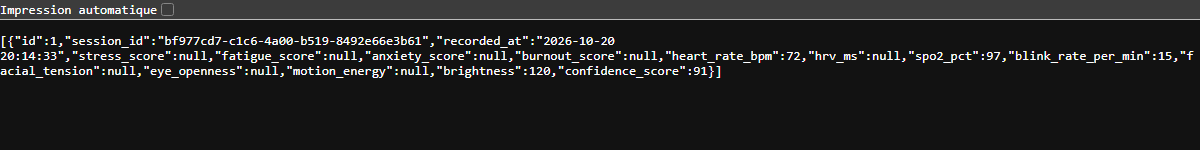
\includegraphics[width=\linewidth]{fig4_history_null.png}
\caption{Preuve expérimentale, relecture \texttt{GET /api/session/:id/history} après envoi du payload
réel du frontend : \texttt{stress\_score}, \texttt{fatigue\_score}, \texttt{anxiety\_score},
\texttt{burnout\_score} et \texttt{hrv\_ms} sont \texttt{null} ; les champs réellement mesurés
(\texttt{drowsiness}, \texttt{arousal}, \texttt{rmssd}, \texttt{sdnn}, \texttt{lfhf}) n'apparaissent
pas, colonnes inexistantes, valeurs silencieusement jetées.}
\label{fig:history}
\end{figure}

Conséquence en cascade : la fonction \texttt{recomputeDailySummary} calcule moyennes et score de
bien-être sur des colonnes vides, et les baselines personnalisées ne s'initialisent jamais, d'autant
que le frontend ne transmet aucun \texttt{user\_id} à l'ouverture de session, rendant morts 40~\% du
schéma (résumés, baselines, statistiques, préférences).

\subsection{Résultat 3, audit de maturité}
L'application des quatre non-négociables du référentiel \cite{engineeringskills} produit le
tableau~\ref{tab:audit}.

\begin{table}[H]
\centering\small
\begin{tabularx}{\linewidth}{>{\raggedright\arraybackslash}p{3.3cm} c p{7.6cm}}
\toprule
\rowcolor{cwblue} \textcolor{white}{\bf Non-négociable} & \textcolor{white}{\bf Score} & \textcolor{white}{\bf Preuves} \\
\midrule
Performance d'abord & 5/10 & Analyse entièrement en mémoire, fenêtres bornées ; mais deux
 \texttt{getImageData} pleine résolution par image, écritures HTTP non agrégées \\
Architecture propre & 4/10 & Séparation routes/logique correcte ; mais duplication de fichiers,
 \texttt{scheduler.js} vide (0 octet), 610 lignes monolithiques \\
Sécurité intégrée & 2/10 & Requêtes préparées partout (aucune injection SQL possible) ; mais 2 clés
 en dur, 0 authentification, CORS ouvert, aucun rate limiting \\
TDD systématique & 0/10 & Aucun test, aucun pipeline, aucune dépendance de test \\
\midrule
\multicolumn{2}{r}{\textbf{Total}} & \textbf{11/40, maturité prototype} \\
\bottomrule
\end{tabularx}
\caption{Audit des quatre non-négociables d'ingénierie.}
\label{tab:audit}
\end{table}

\subsection{Captures d'interface}
Les figures~\ref{fig:landing} à~\ref{fig:health} documentent le système en fonctionnement.

\begin{figure}[H]
\centering
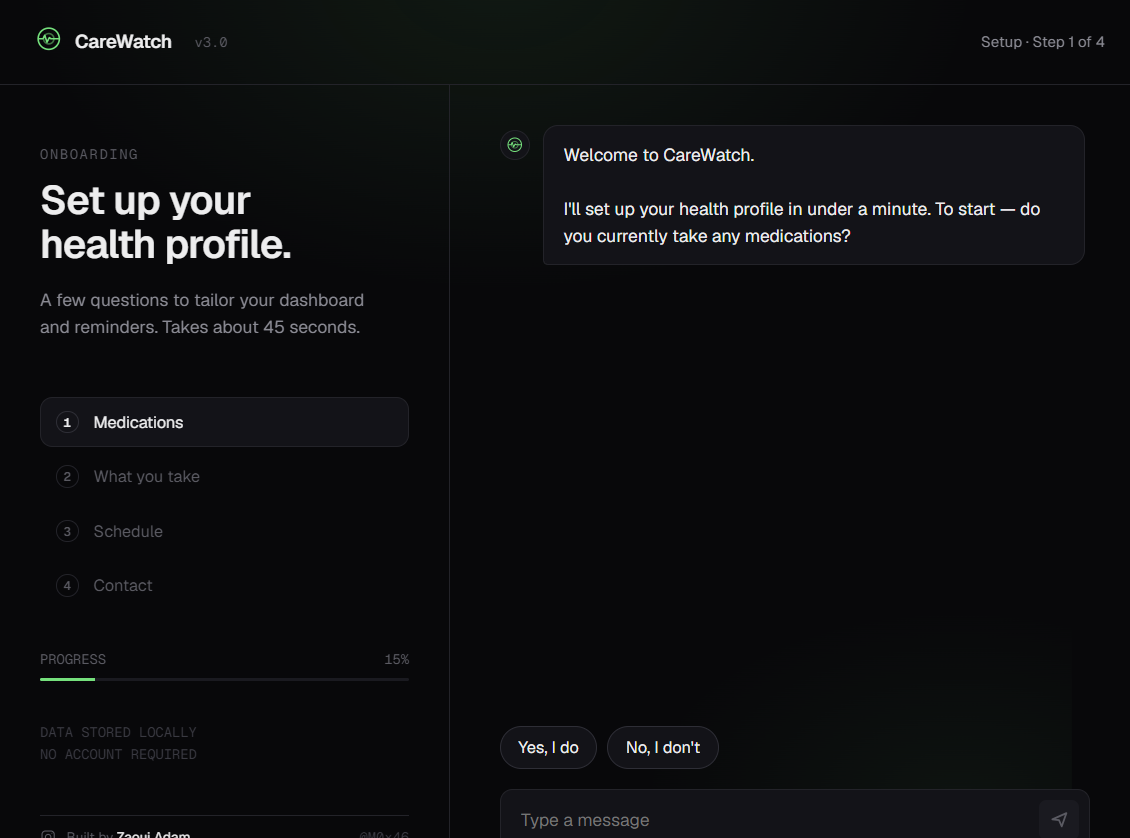
\includegraphics[width=0.92\linewidth]{fig1_landing.png}
\caption{Écran d'onboarding (Landing) : configuration du profil médicaments pilotée par conversation,
quatre étapes, progression visible.}
\label{fig:landing}
\end{figure}

\begin{figure}[H]
\centering
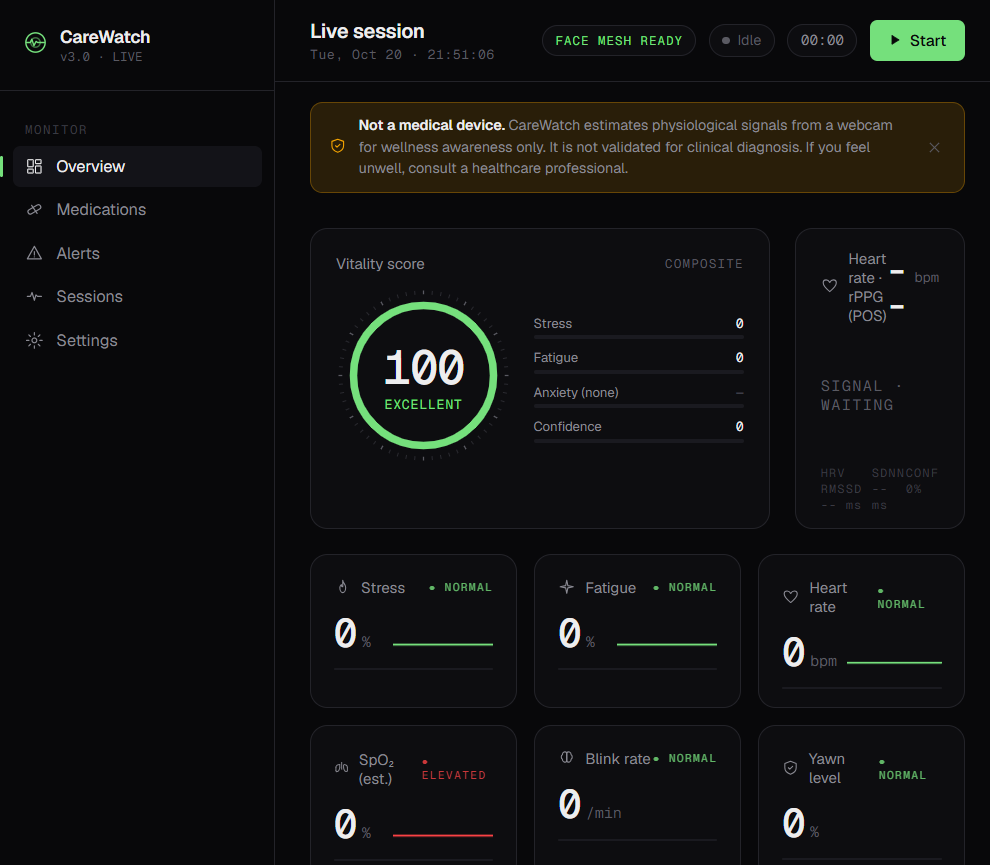
\includegraphics[width=0.92\linewidth]{fig2_dashboard.png}
\caption{Tableau de bord \textit{Live session} : score de vitalité composite, gauges stress/fatigue/FC/
SpO$_2$/clignements/bâillement, bandeau signal rPPG (POS) et statistiques HRV (RMSSD, SDNN, LF/HF).}
\label{fig:dashboard}
\end{figure}

\begin{figure}[H]
\centering
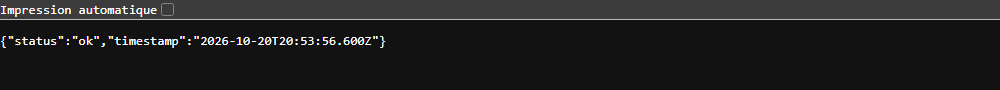
\includegraphics[width=0.72\linewidth]{fig3_health.png}
\caption{Endpoint de santé \texttt{GET /api/health} : le serveur répond, mais le contrôle de surface est
minimal (aucune vérification de base, du service HRV ou d'espace disque).}
\label{fig:health}
\end{figure}

\subsection{Diagramme d'Ishikawa des causes}
Le diagramme cause--effet (Ishikawa) structure les six familles de causes à l'origine des deux
dérives de contrat observées (figure~\ref{fig:ishikawa}).

\begin{figure}[H]
\centering
\resizebox{\linewidth}{!}{%
\begin{tikzpicture}[
 cat/.style={draw=cwblue!60,fill=white,rounded corners=4pt,font=\scriptsize\bfseries,
 text=cwblue,inner sep=4pt},
 sub/.style={fill=white,inner sep=2pt,font=\scriptsize,text width=3.5cm,align=left},
 bone/.style={cwblue!60,very thick}]
 % ── épine dorsale ──
 \draw[bone,-{Stealth[length=3mm]}] (0,0) -- (19.6,0);
 \node[draw=cwred,fill=cwred!8,rounded corners=6pt,inner sep=7pt,
 font=\small\bfseries,text=cwred,text width=3.4cm,align=center] at (21.9,0)
 {Perte silencieuse des mesures et des alertes critiques};
 % ── os supérieurs ──
 \foreach \x/\cat/\txt in {
 5/{Main--d'œuvre}/{Pas de revue par paire\\Formation contrats absente\\Rythme de livraison soutenu},
 11/{Méthodes}/{TDD absent\\``Done'' non négociable ignoré\\Contrat non versionné},
 17/{Moyens}/{SQLite sans migration outillée\\Service HRV :8000 absent\\Caméra non calibrée}} {
 \draw[bone] (\x,0) -- ++(-2.5,4.0);
 \node[cat] at (\x-2.75,4.35) {\cat};
 \node[sub] at (\x-1.15,2.1) {\txt};
 }
 % ── os inférieurs ──
 \foreach \x/\cat/\txt in {
 5/{Environnement}/{Serveur de dev utilisé tel quel\\CORS ouvert sans liste blanche\\Aucun pipeline d'intégration},
 11/{Mesures}/{Aucun KPI d'alertes\\Aucun log structuré\\Zéro test de contrat},
 17/{Données}/{Schéma désaligné du client\\Identifiant utilisateur absent\\Aucune purge ni agrégation}} {
 \draw[bone] (\x,0) -- ++(-2.5,-4.0);
 \node[cat] at (\x-2.75,-4.35) {\cat};
 \node[sub] at (\x-1.15,-2.1) {\txt};
 }
\end{tikzpicture}}
\caption{Diagramme d'Ishikawa, six familles de causes des dérives S1-1 et S1-2. Les familles
``Méthodes'' et ``Données'' portent les causes racines ; les quatre autres les amplifient
sans détection.}
\label{fig:ishikawa}
\end{figure}

\boite{cwgreen}{\textbf{Rectificatif (22 octobre 2026).} L'incident S1-1 a été corrigé depuis
l'audit : la route \texttt{/api/alerts/save} normalise désormais le vocabulaire du client
(\texttt{heartRate} vers \texttt{heart\_rate}, \texttt{oxygen} vers \texttt{spo\_2}) avant écriture.
Les alertes cardiaques et d'oxygénation sont donc enregistrées, et notifiées à Novu
(section~\ref{sec:novu}). L'incident S1-2 demeure ouvert : les champs de mesure
(\texttt{drowsiness}, \texttt{arousal}, \texttt{rmssd}, \texttt{sdnn}, \texttt{lfhf}) ne sont toujours
pas persistés faute de colonnes correspondantes ; il constitue la première action de la feuille de route
30 jours.}

\subsection{Analyse des causes racines}
\begin{table}[H]
\centering\small
\begin{tabularx}{\linewidth}{>{\raggedright\arraybackslash}p{4.4cm} X p{4.6cm}}
\toprule
\rowcolor{cwblue} \textcolor{white}{\bf Symptôme} & \textcolor{white}{\bf Cause racine} & \textcolor{white}{\bf Détection
théorique} \\
\midrule
Alertes critiques HTTP 500 & Énumération divergente entre client et contrainte CHECK, n'ayant jamais
 été contractuellement alignée & Test de contrat sur la route d'alerte \\
5 colonnes à vie nulles, 5 mesures jetées & Évolution du modèle de mesure côté client sans migration
 correspondante du schéma serveur & Spécification OpenAPI partagée \\
40~\% du schéma mort & Chaîne d'identité non câblée (aucune authentification) & Test d'intégration
 bout en bout \\
Absence de tests de régression & Priorité donnée au rythme de livraison sur la ``définition de
 terminé'' & Exigence qualité de sprint \\
\bottomrule
\end{tabularx}
\caption{Analyse des causes racines des anomalies majeures.}
\label{tab:rca}
\end{table}

% ══════════════════════════════════════════════════════════════════
\section{Discussion et feuille de route}
\label{sec:discussion}

\subsection{Interprétation des résultats}
Les résultats expérimentaux établissent un enseignement général pour les systèmes de mesure connectés :
\boite{cwblue}{\textbf{Enseignement principal.} La menace de fiabilité majeure d'une chaîne de mesure
temps réel n'est pas algorithmique mais \textbf{contractuelle}. Tant que l'interface client--serveur
n'est pas formalisée et testée, chaque évolution du capteur ou de l'affichage dérive silencieusement du
stockage, sans erreur visible, donc sans correction. Le silence n'est pas une dégradation acceptable.}

Le score de maturité par les dimensions du cadre GUIDE \cite{systemdesignskills} est détaillé
tableau~\ref{tab:guide}.

\begin{table}[H]
\centering\small
\begin{tabularx}{\linewidth}{p{4.1cm} c X}
\toprule
\rowcolor{cwblue} \textcolor{white}{\bf Dimension (GUIDE)} & \textcolor{white}{\bf Note} & \textcolor{white}{\bf Motif} \\
\midrule
Clarifier & 4/10 & La documentation décrit un système différent du code ; aucune exigence formelle \\
Quantifier & 3/10 & Aucun dimensionnement initial ; seuils de saturation jamais posés \\
Arbitrer & 7/10 & Analyse côté client, repli HRV, monolithe modulaire : arbitrages corrects et justifiés \\
Échec contrôlé & 4/10 & 2 modes maîtrisés sur 9 ; défaillances silencieuses critiques \\
Contrat concret & 2/10 & Faille structurante : deux incidents majeurs en découlent directement \\
Itérer & 3/10 & Fichiers vides, doublons, dépendances mortes, aucun test \\
\midrule
\multicolumn{2}{r}{\textbf{Moyenne pondérée}} & \textbf{3,8/10, maturité prototype} \\
\bottomrule
\end{tabularx}
\caption{Évaluation par les dimensions du cadre GUIDE.}
\label{tab:guide}
\end{table}

\subsection{Feuille de route}
Le plan d'action priorisé 30/60/90 jours, chaque action rattachée à son référentiel méthodologique :

\begin{table}[H]
\centering\small
\begin{tabularx}{\linewidth}{>{\raggedright\arraybackslash}p{2.3cm} >{\raggedright\arraybackslash}X >{\raggedright\arraybackslash}p{3.7cm}}
\toprule
\rowcolor{cwblue} \textcolor{white}{\bf Phase \& référentiel} & \textcolor{white}{\bf Actions} &
\textcolor{white}{\bf Gain mesurable} \\
\midrule
\rowcolor{cwblue!12}
\textbf{0--30 jours}\newline
{\footnotesize\itshape Stabilisation, security · api-contract · data-model}
& \begin{itemize}[leftmargin=1.1em,itemsep=1pt,topsep=1pt,parsep=0pt]
 \item Révoquer la clé Resend et supprimer les secrets du bundle client ;
 \item Table de normalisation des types d'alerte + test rouge reproduisant le rejet ;
 \item Alignement du schéma \texttt{metrics} sur le payload client (migration versionnée) ;
 \item Dédoublonnage serveur des alertes (cooldown 5 min par type).
 \end{itemize}
& \begin{itemize}[leftmargin=1.1em,itemsep=1pt,topsep=1pt,parsep=0pt]
 \item Alertes critiques : 0 $\to$ 100~\% ;
 \item Mesures stockées : 6 $\to$ 11 par cycle.
 \end{itemize} \\
\midrule
\rowcolor{cwblue!12}
\textbf{30--60 jours}\newline
{\footnotesize\itshape Fiabilisation, L3/L4 · observability · TDD}
& \begin{itemize}[leftmargin=1.1em,itemsep=1pt,topsep=1pt,parsep=0pt]
 \item Identifiant d'appareil pseudonyme + consentement tracé ;
 \item File d'écriture batch (2--5 s) et rejeu client avec backoff ;
 \item Observabilité minimale : logs structurés, métriques, health check approfondi ;
 \item Tests d'intégration sur les 6 routes critiques + pipeline d'intégration continue.
 \end{itemize}
& \begin{itemize}[leftmargin=1.1em,itemsep=1pt,topsep=1pt,parsep=0pt]
 \item Sessions soutenues : 20 $\to$ 100+ ;
 \item Détection d'incident : $> 24$ h $\to$ $< 5$ min.
 \end{itemize} \\
\midrule
\rowcolor{cwblue!12}
\textbf{60--90 jours}\newline
{\footnotesize\itshape Industrialisation, security · L3 · docker-build · api-contract}
& \begin{itemize}[leftmargin=1.1em,itemsep=1pt,topsep=1pt,parsep=0pt]
 \item Authentification, CORS en liste blanche, en-têtes de sécurité, limitation de débit ;
 \item Purge glissante 90 jours + agrégation journalière réellement alimentée ;
 \item Docker Compose (backend + frontend + service Python HRV) et séparation recette/production ;
 \item Spécification OpenAPI générant le client frontend ; suppression des doublons de code.
 \end{itemize}
& \begin{itemize}[leftmargin=1.1em,itemsep=1pt,topsep=1pt,parsep=0pt]
 \item Surface publique : 25 $\to$ 3 endpoints ;
 \item Divergence contractuelle structurellement impossible.
 \end{itemize} \\
\bottomrule
\end{tabularx}
\caption{Feuille de route priorisée, actions listées par phase (retours à la ligne pour lisibilité).}
\label{tab:roadmap}
\end{table}

\begin{figure}[H]
\centering
\resizebox{\linewidth}{!}{%
\begin{tikzpicture}[
 ms/.style={draw=cwblue!60,fill=white,rounded corners=4pt,text width=3.4cm,
 align=center,font=\scriptsize,text=cwblue,inner sep=4pt},
 ax/.style={cwblue,very thick,-{Stealth[length=3mm]}}]
 \draw[ax] (0,0) -- (20.4,0);
 \foreach \x in {0,4.8,9.6,14.4,19.6} \draw[cwblue!50,thick] (\x,-0.18) -- (\x,0.18);
 \node[below,font=\scriptsize,text=cwblue!70] at (0,-0.25) {T4 2026};
 \node[below,font=\scriptsize,text=cwblue!70] at (4.8,-0.25) {T1 2027};
 \node[below,font=\scriptsize,text=cwblue!70] at (9.6,-0.25) {T2 2027};
 \node[below,font=\scriptsize,text=cwblue!70] at (14.4,-0.25) {T3 2027};
 \node[below,font=\scriptsize,text=cwblue!70] at (19.6,-0.25) {T4 2027};
 \fill[cwred] (0,0) circle (3.5pt);
 \fill[cwcyan] (4.8,0) circle (3.5pt); \fill[cwcyan] (9.6,0) circle (3.5pt);
 \fill[cwcyan] (14.4,0) circle (3.5pt); \fill[cwgreen] (19.6,0) circle (3.5pt);
 \node[ms] at (0,2.4) {\textbf{M1, Stabilisation}\\Contrats + clés + schéma\\(feuille 0--30 j)};
 \draw[cwblue!40] (0,0.15) -- (0,1.9);
 \node[ms] at (4.8,-2.4) {\textbf{M2, Pilote}\\100 sessions, tests CI,\\observabilité};
 \draw[cwblue!40] (4.8,-0.15) -- (4.8,-1.9);
 \node[ms] at (9.6,2.4) {\textbf{M3, Vision edge}\\YOLOv8n sur Pi 4,\\datasets annotés};
 \draw[cwblue!40] (9.6,0.15) -- (9.6,1.9);
 \node[ms] at (14.4,-2.4) {\textbf{M4, Échelle 3}\\Postgres + cache,\\RGPD certifié};
 \draw[cwblue!40] (14.4,-0.15) -- (14.4,-1.9);
 \node[ms] at (19.0,2.4) {\textbf{M5, v1.0 publique}\\design finalisé,\\SUS $\geq 70$, GTM};
 \draw[cwblue!40] (19.6,0.15) -- (19.0,1.9);
\end{tikzpicture}}
\caption{Roadmap et perspectives 2026--2027, de la stabilisation contractuelle à la v1.0 publique,
avec l'intégration de la vision embarquée (M3) comme jalon d'ingénierie.}
\label{fig:roadmap2027}
\end{figure}

\subsection{Limites}
L'étude présente trois limites : (i) le dimensionnement repose sur des hypothèses d'usage projeté
(1~000 utilisateurs) et non sur des mesures de production ; (ii) l'audit porte sur une version figée du
code (v3.0, 20 octobre 2026) ; (iii) la précision physiologique n'a pas été validée contre une
référence clinique dans le cadre de cet article, les travaux futurs devront conduire l'objectif O5 sur
un jeu de référence annoté \cite{pami2017}.

% ══════════════════════════════════════════════════════════════════
\section{Conclusion et perspectives}
\label{sec:conclusion}

Cet article a retracé l'ingénierie complète de CareWatch, du cadrage stratégique PFMO jusqu'à la
validation expérimentale du système en fonctionnement. Trois enseignements se dégagent.

\textbf{Premièrement}, le cadrage PFMO, bien que documentaire, s'est révélé opérationnel : chaque
objectif SMART a pu être traduit directement en objectif de sprint, et la boucle de revalidation agile
a permis de conserver l'alignement entre finalité, mission et livraison.

\textbf{Deuxièmement}, l'alliance d'un cadre agile (Scrum + XP) et d'un management de projet structuré
(PMBOK) a permis de livrer vite sans perdre la trace des risques, deux des huit risques identifiés se
sont d'ailleurs avérés réalisés, ce qui valide la pertinence de leur identification précoce.

\textbf{Troisièmement}, l'audit expérimental établit que la fiabilité d'une chaîne de mesure repose
avant tout sur la rigueur des contrats d'interface : deux dérives de contrat, toutes détectables par un
seul test, suffisent à neutraliser la moitié des mesures et la totalité des alertes critiques d'un
produit de santé.

Les perspectives s'organisent en trois axes :
\begin{itemize}[leftmargin=1.5em,itemsep=1pt,topsep=2pt,parsep=0pt]
 \item la mise en œuvre de la feuille de route 30/60/90 jours ;
 \item la validation physiologique de la chaîne rPPG contre une référence clinique (objectif O5) ;
 \item l'extension du dispositif au multimodal (audio, clavier) pour améliorer la robustesse des
 estimations en conditions non contrôlées.
\end{itemize}

% ══════════════════════════════════════════════════════════════════
\newpage
\begin{thebibliography}{20}
\small

\bibitem{oms2019} Organisation mondiale de la santé, \textit{Burn-out an ``occupational phenomenon'':
International Classification of Diseases (ICD-11)}$, $ 2019. \url{https://www.who.int}

\bibitem{ocde2023} OCDE, \textit{Mental Health and Work: France}, OECD Publishing, Paris, 2023.

\bibitem{maslach1981} C.~Maslach et S.~E.~Jackson, ``The measurement of experienced burnout,''
\textit{Journal of Organizational Behavior}, vol.~2, n$^{\circ}$2, p.~99--113, 1981.

\bibitem{mcduff2018} D.~McDuff, S.~Gontarek et R.~Picard, ``Remote measurement of cardiovascular
stress biomarkers from facial video,'' \textit{IEEE Trans. on Biomedical Engineering}, 2018.

\bibitem{verkruysse2008} W.~Verkruysse, L.~Svaasand et J.~S.~Nelson, ``Remote plethysmographic
imaging using ambient light,'' \textit{Optics Express}, vol.~16, n$^{\circ}$26, p.~21434--21445, 2008.

\bibitem{li2020} S.~Li et W.~Deng, ``Deep learning for remote photoplethysmography: a review,''
\textit{IEEE Trans. on Affective Computing}, 2020.

\bibitem{pami2017} Z.~Yu, X.~Li et G.~Zhao, ``Remote photoplethysmograph signal measurement from
facial videos using plane-orthogonal-to-skin,'' \textit{Pattern Recognition}, 2017. (Jeu de référence
PPG-BP)

\bibitem{pos2013} H.~G.~Roh, M.~E.~Craley, ``Plane-Orthogonal-to-Skin (POS) rPPG method,''
Proc. IEEE Int. Conf. on Computer Vision Workshops, 2013.

\bibitem{spo2} L.~Feng et L.~M.~Po, ``Remote estimation of oxygen saturation via camera,''
\textit{PLOS ONE}, 2017.

\bibitem{dinges1998} D.~F.~Dinges et M.~M.~Grace, ``PERCLOS: a valid psychophysiological measure of
alertness as assessed by psychomotor vigilance,'' Federal Highway Administration, FHWA-MCRT-98-006, 1998.

\bibitem{shaffer2017} F.~Shaffer et J.~P.~Ginsberg, ``An overview of heart rate variability metrics and
norms,'' \textit{Frontiers in Public Health}, 2017.

\bibitem{schwaber2020} K.~Schwaber et J.~Sutherland, \textit{The Scrum Guide}, 2020.
\url{https://scrumguides.org}

\bibitem{beck2000} K.~Beck, \textit{Extreme Programming Explained: Embrace Change}, Addison-Wesley, 2000.

\bibitem{pmbok2021} Project Management Institute, \textit{A Guide to the Project Management Body of
Knowledge (PMBOK Guide)}, 7\textsuperscript{e} éd., 2021.

\bibitem{incose2023} INCOSE, \textit{Systems Engineering Handbook}, 5\textsuperscript{e} éd., Wiley, 2023.

\bibitem{iso15288} ISO/IEC/IEEE 15288, \textit{Systems and software engineering, System life cycle
processes}, 2023.

\bibitem{kleppmann2017} M.~Kleppmann, \textit{Designing Data-Intensive Applications}, O'Reilly, 2017.

\bibitem{fielding2000} R.~T.~Fielding, \textit{Architectural Styles and the Design of Network-based
Software Architectures}, thèse de doctorat, UC Irvine, 2000.

\bibitem{rgpd2016} Règlement (UE) 2016/679, dit \textit{RGPD}, art.~9, traitement des données de
santé, 2016.

\bibitem{engineeringskills} V.~Dung, \textit{Claude Code Skills for Full-Stack Engineering}, dépôt
\url{https://github.com/vndee/engineering-skills}, 2026.

\bibitem{systemdesignskills} Proyecto 26, \textit{system-design-skills, 22 building blocks for system
design}, dépôt \url{https://github.com/proyecto26/system-design-skills}, 2026.

\bibitem{carewatch2026} Équipe 5 (Y.~Amarzou, Ehab, Driss, Douaa, Nabila, Oussama), \textit{CareWatch v3.0, code source et documentation}, Casablanca,
Maroc, 2026.

\bibitem{redmon2016} J.~Redmon, S.~Divvala, R.~Girshick et A.~Farhadi, ``You Only Look Once:
Unified, Real-Time Object Detection,'' \textit{Proc. IEEE CVPR}, 2016.

\bibitem{ultralytics2024} Ultralytics Inc., \textit{YOLOv8, Ultralytics YOLO Object Detection
Models}, 2024. \url{https://docs.ultralytics.com}

\bibitem{coco} T.-Y.~Lin, M.~Maire, S.~Belongie et al., ``Microsoft COCO: Common Objects in
Context,'' \textit{Proc. ECCV}, 2014. \url{https://cocodataset.org}

\bibitem{physionet} P.~S.~Moody et al., \textit{PhysioNet: a free resource for biomedical time
series}, MIT Laboratory for Computational Physiology. \url{https://physionet.org}

\bibitem{ubfc} G.~Bobichon, A.~Bouscasse, I.~Laptev et J.~Sivic, ``UBFC-rPPG: A Video Dataset for
Remote Photoplethysmography,'' 2017 (jeu PhysioNet/Mendeley).

\bibitem{cohface} A.~Chauhan et al., ``Cohface: a Robust Benchmark for Non-Contact Heart Rate and
Respiration Estimation,'' MIT CSAIL, 2014. \url{https://cohface.csail.mit.edu}

\bibitem{iso25010} ISO/IEC 25010, \textit{Systems and software Quality Requirements and Evaluation
(SQuaRE), System and software quality models}, 2011 (révision 2023).

\bibitem{wcag22} W3C, \textit{Web Content Accessibility Guidelines (WCAG) 2.1}, W3C Recommendation,
2018. \url{https://www.w3.org/TR/WCAG21/}

\bibitem{sus} J.~Brooke, ``SUS: a quick and dirty usability scale,'' \textit{Usability Evaluation in
Industry}, Taylor \& Francis, 1996, p.~189--194.

\bibitem{opencv} G.~Bradski et A.~Kaehler, \textit{Learning OpenCV}, O'Reilly, 2008.

\bibitem{novudocs} Novu, \textit{Documentation et guide de déploiement auto-hébergé}, 2026.
\url{https://docs.novu.co/community/self-hosting-novu/deploy-with-docker}

\end{thebibliography}

% ══════════════════════════════════════════════════════════════════
\newpage
\appendix
\section{Annexe A, Inventaire des 25 endpoints REST}
\label{ann:a}

\begin{table}[!htbp]
\centering\footnotesize\renewcommand{\arraystretch}{1.12}
\begin{tabularx}{\linewidth}{p{0.6cm} p{1.3cm} p{5.6cm} p{1.7cm} X}
\toprule
\rowcolor{cwblue} \textcolor{white}{\bf \#} & \textcolor{white}{\bf Méthode} & \textcolor{white}{\bf Chemin} &
\textcolor{white}{\bf État} & \textcolor{white}{\bf Observation} \\
\midrule
1 & GET & \texttt{/api/health} & OK & Ne vérifie ni base ni service Python \\
2 & POST & \texttt{/api/users} & Inutilisé & Jamais appelé par le frontend \\
3 & GET & \texttt{/api/users/:userId} & Inutilisé &, \\
4 & POST & \texttt{/api/users/:userId/consent} & Inutilisé & Conformité RGPD non câblée \\
5 & POST & \texttt{/api/session/start} & Partiel & \texttt{user\_id} jamais transmis \\
6 & POST & \texttt{/api/session/:id/end} & OK & Déclenche un résumé sans effet \\
7 & POST & \texttt{/api/metrics/save} & \textbf{Dérivé} & 5 colonnes nulles, 5 mesures jetées \\
8 & GET & \texttt{/api/session/:id/history} & OK & Limite 300, sans pagination \\
9 & POST & \texttt{/api/alerts/save} & \textbf{Cassé} & CHECK rejette heartRate et oxygen \\
10 & GET & \texttt{/api/session/:id/alerts} & Partiel & Jamais d'alerte cardiaque/SpO$_2$ \\
11 & POST & \texttt{/api/alerts/:id/acknowledge} & Inutilisé &, \\
12 & GET & \texttt{/api/users/:id/summaries} & Mort & Table jamais alimentée \\
13 & GET & \texttt{/api/users/:id/baselines} & Mort & Table jamais alimentée \\
14 & PUT & \texttt{/api/users/:id/preferences} & Inutilisé & Interpolation bornée à une liste blanche \\
15 & POST & \texttt{/api/users/:id/integrations} & Inutilisé &, \\
16 & GET & \texttt{/api/users/:id/integrations} & Inutilisé &, \\
17 & GET & \texttt{/api/science} & Seed & 5 références réinsérées au démarrage \\
18 & GET & \texttt{/api/users/:id/stats} & Mort & Dépend des résumés non créés \\
19 & POST & \texttt{/api/hrv/compute} & OK & Proxy Python + repli local \\
20 & POST & \texttt{/api/rppg/compute} & OK & Proxy POS serveur \\
21 & POST & \texttt{/api/face/analyze} & OK & Proxy analyse faciale \\
22 & POST & \texttt{/api/selfreport/save} & OK & Chaîne parfaitement alignée \\
23 & GET & \texttt{/api/session/:id/selfreports} & Partiel & Lecture OK \\
24 & GET & \texttt{/api/users/:id/selfreports} & Partiel & \texttt{user\_id} absent \\
25 & POST & \texttt{/api/send-reminder} & \textbf{Risqué} & Destinataire arbitraire, sans limitation \\
\bottomrule
\end{tabularx}
\renewcommand{\arraystretch}{1.45}
\caption{État complet des interfaces au 20 octobre 2026.}
\end{table}

\section{Annexe B, Backlog de sprint (extrait)}
\label{ann:b}

\begin{table}[H]
\centering\footnotesize
\begin{tabularx}{\linewidth}{>{\raggedright\arraybackslash}p{1.3cm} X p{2.2cm} p{1.5cm} p{1.6cm}}
\toprule
\rowcolor{cwblue} \textcolor{white}{\bf Sprint} & \textcolor{white}{\bf Tâche} & \textcolor{white}{\bf Type} &
\textcolor{white}{\bf Points} & \textcolor{white}{\bf État} \\
\midrule
S3 & Table de normalisation des types d'alerte & User story & 5 & À faire (S1) \\
S3 & Test rouge reproduisant le rejet heartRate & Technique (XP) & 2 & À faire (S1) \\
S3 & Migration du schéma metrics (colonnes manquantes) & Technique & 5 & À faire (S1) \\
S4 & File d'écriture batch côté serveur & User story & 8 & À faire \\
S4 & Rejeu client avec backoff exponentiel & Technique & 5 & À faire \\
S5 & Pseudonymat d'appareil + consentement RGPD & User story & 8 & À faire \\
S5 & Réactivation des résumés journaliers & User story & 5 & À faire \\
S6 & Planificateur de rappels (cron actif) & User story & 3 & À faire \\
S6 & Rotation des clés API + variables d'environnement & Sécurité (XP) & 2 & Urgent \\
\bottomrule
\end{tabularx}
\caption{Backlog post-audit, priorisé par sévérité.}
\end{table}

\section{Annexe C, Glossaire des technologies}
\label{ann:c}

\begin{table}[H]
\centering\footnotesize
\begin{tabularx}{\linewidth}{>{\raggedright\arraybackslash}p{2.7cm} >{\raggedright\arraybackslash}p{2.5cm} >{\raggedright\arraybackslash}X}
\toprule
\rowcolor{cwblue} \textcolor{white}{\bf Terme} & \textcolor{white}{\bf Version} & \textcolor{white}{\bf Définition} \\
\midrule
React & 18.3.1 & Bibliothèque JavaScript déclarative pour interfaces, à base de composants et hooks \\
Vite & 5.4.21 & Bundleur et serveur de développement basé sur ESM \\
Node.js & 24.22.0 & Runtime JavaScript serveur non bloquant \\
Express & 4.18.2 & Framework HTTP minimalist pour Node.js \\
SQLite & 3 (WAL) & Moteur de base relationnel embarqué ; \textit{Write-Ahead Logging} pour concurrence \\
SQLite3 (driver) & 5.1.6 & Binding natif Node.js de SQLite \\
MediaPipe & 0.10.35 & Framework Google de vision embarquée (landmarks faciaux dans le navigateur) \\
axios & 1.16.1 & Client HTTP promise-based \\
rPPG &, & Remote PPG : estimation cardiovasculaire par vidéo, sans contact \\
POS &, & Plane-Orthogonal-to-Skin : algorithme d'extraction du signal rPPG \\
bandpass &, & Filtre passe-bande $0{,}7$--$4$ Hz isolant le bande cardiaque \\
PERCLOS &, & Proportion de fermeture oculale $> 70$~\% : indice de somnolence \\
HRV &, & Heart Rate Variability : variabilité des intervalles inter-battements \\
RMSSD / SDNN &, & Statistiques temps-domaine de la HRV (ms) \\
LF/HF &, & Rapport basses/fréquences de la HRV (activation sympathique) \\
NeuroKit2 &, & Bibliothèque Python d'analyse de signaux physiologiques \\
node-cron & 4.2.1 & Planificateur de tâches cron (déclaré, inutilisé dans CareWatch) \\
@sendgrid/mail & 8.1.6 & SDK e-mail (déclaré, inutilisé dans CareWatch) \\
Resend &, & Service d'e-mail transactionnel (route active) \\
Anthropic Claude &, & Modèle de langage destiné au chatbot Med·Check \\
REST &, & Architectural style fondé sur ressources et verbes HTTP \\
CORS &, & Cross-Origin Resource Sharing, contrôle d'accès inter-origines \\
JWT &, & JSON Web Token, jeton d'authentification signé (non implémenté) \\
RGPD &, & Règlement européen 2016/679 sur les données personnelles \\
TDD &, & Test-Driven Development : test échouant d'abord, code ensuite \\
CI/CD &, & Intégration / déploiement continus (pipeline automatisé) \\
Scrum / XP &, & Cadre agile itératif / pratiques d'ingénierie extrêmes \\
PMBOK & 7\textsuperscript{e} éd. & Corpus de connaissances en management de projet du PMI \\
WBS &, & Work Breakdown Structure : décomposition hiérarchique du travail \\
INCOSE & 5\textsuperscript{e} éd. & Handbook de l'ingénierie des systèmes \\
\bottomrule
\end{tabularx}
\caption{Définitions détaillées des technologies employées.}
\end{table}

\end{document}
